\chapter{Kinematics}\label{c:K}

\section{Specific Jet Feature Distributions}

	For the standard set of jet features, plot the overall distributions in a standard 2 hist ratio plot for data and MC. This also includes jet counts possibly


\section{Specific Jet Feature Distributions}

	\subsection{Two Central Channel}
	
		\subsubsection{\pt}
		
			\begin{figure}[h]
				\centering
				
				\begin{minipage}[h]{0.33\linewidth}
					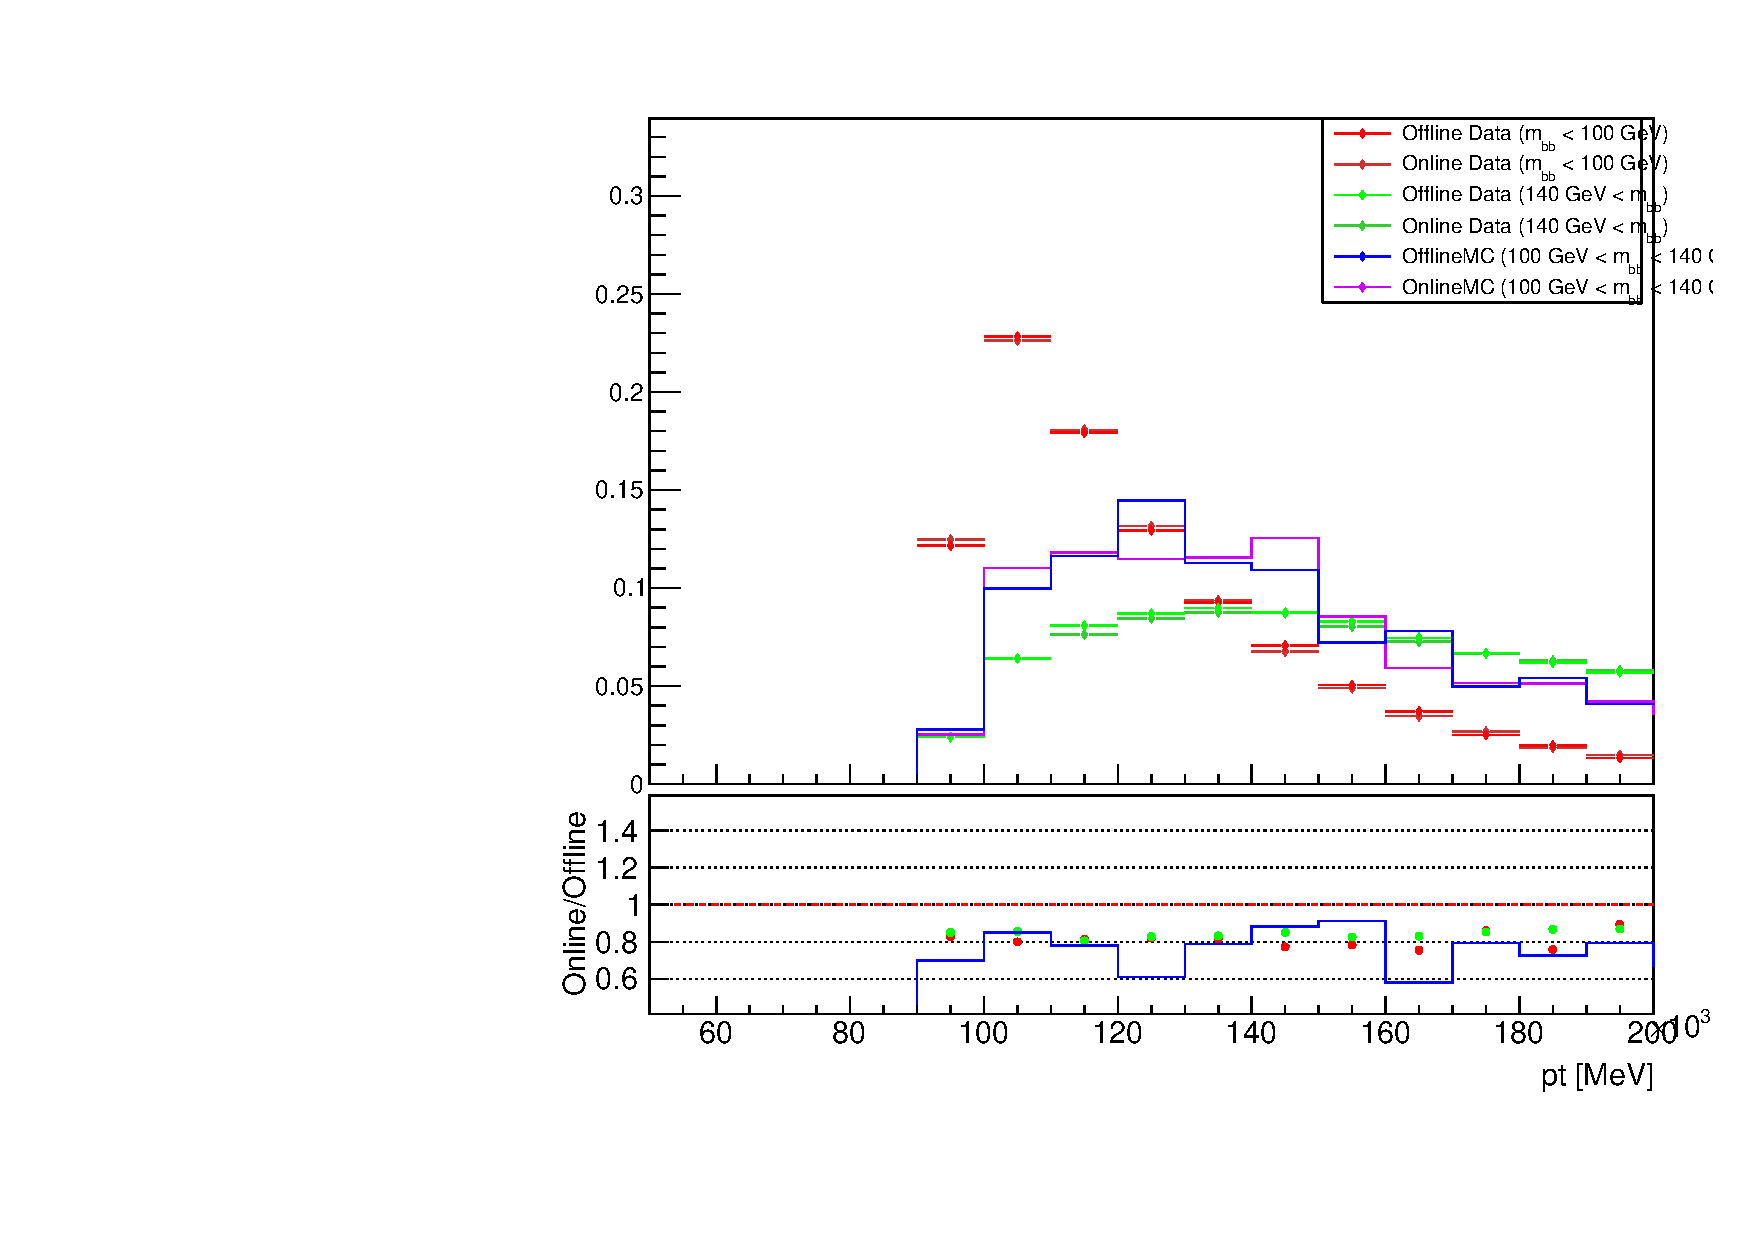
\includegraphics[width=1\linewidth]{pt_bJet1}
				\end{minipage}
				\quad
				\begin{minipage}[h]{0.33\linewidth}
					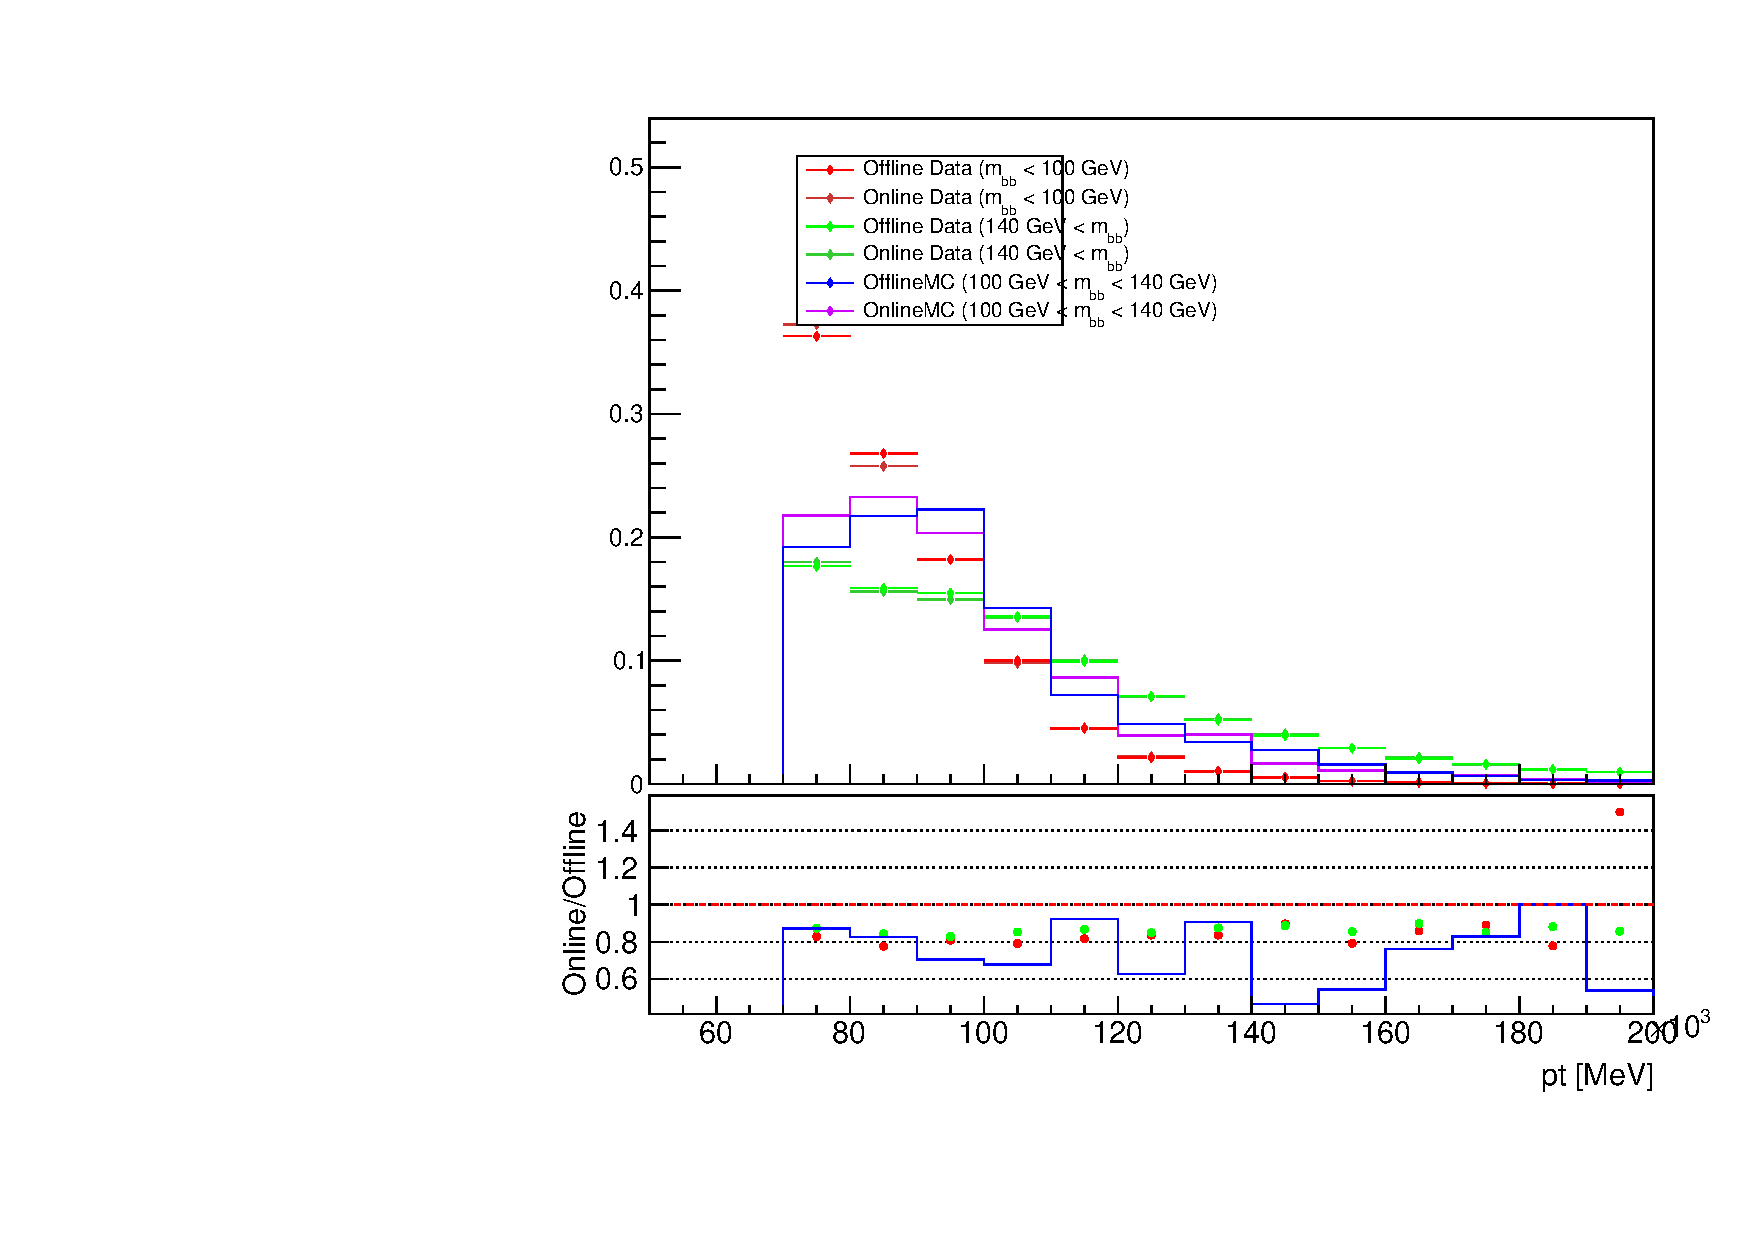
\includegraphics[width=1\linewidth]{pt_bJet2}
				\end{minipage}

				\begin{minipage}[h]{0.33\linewidth}
					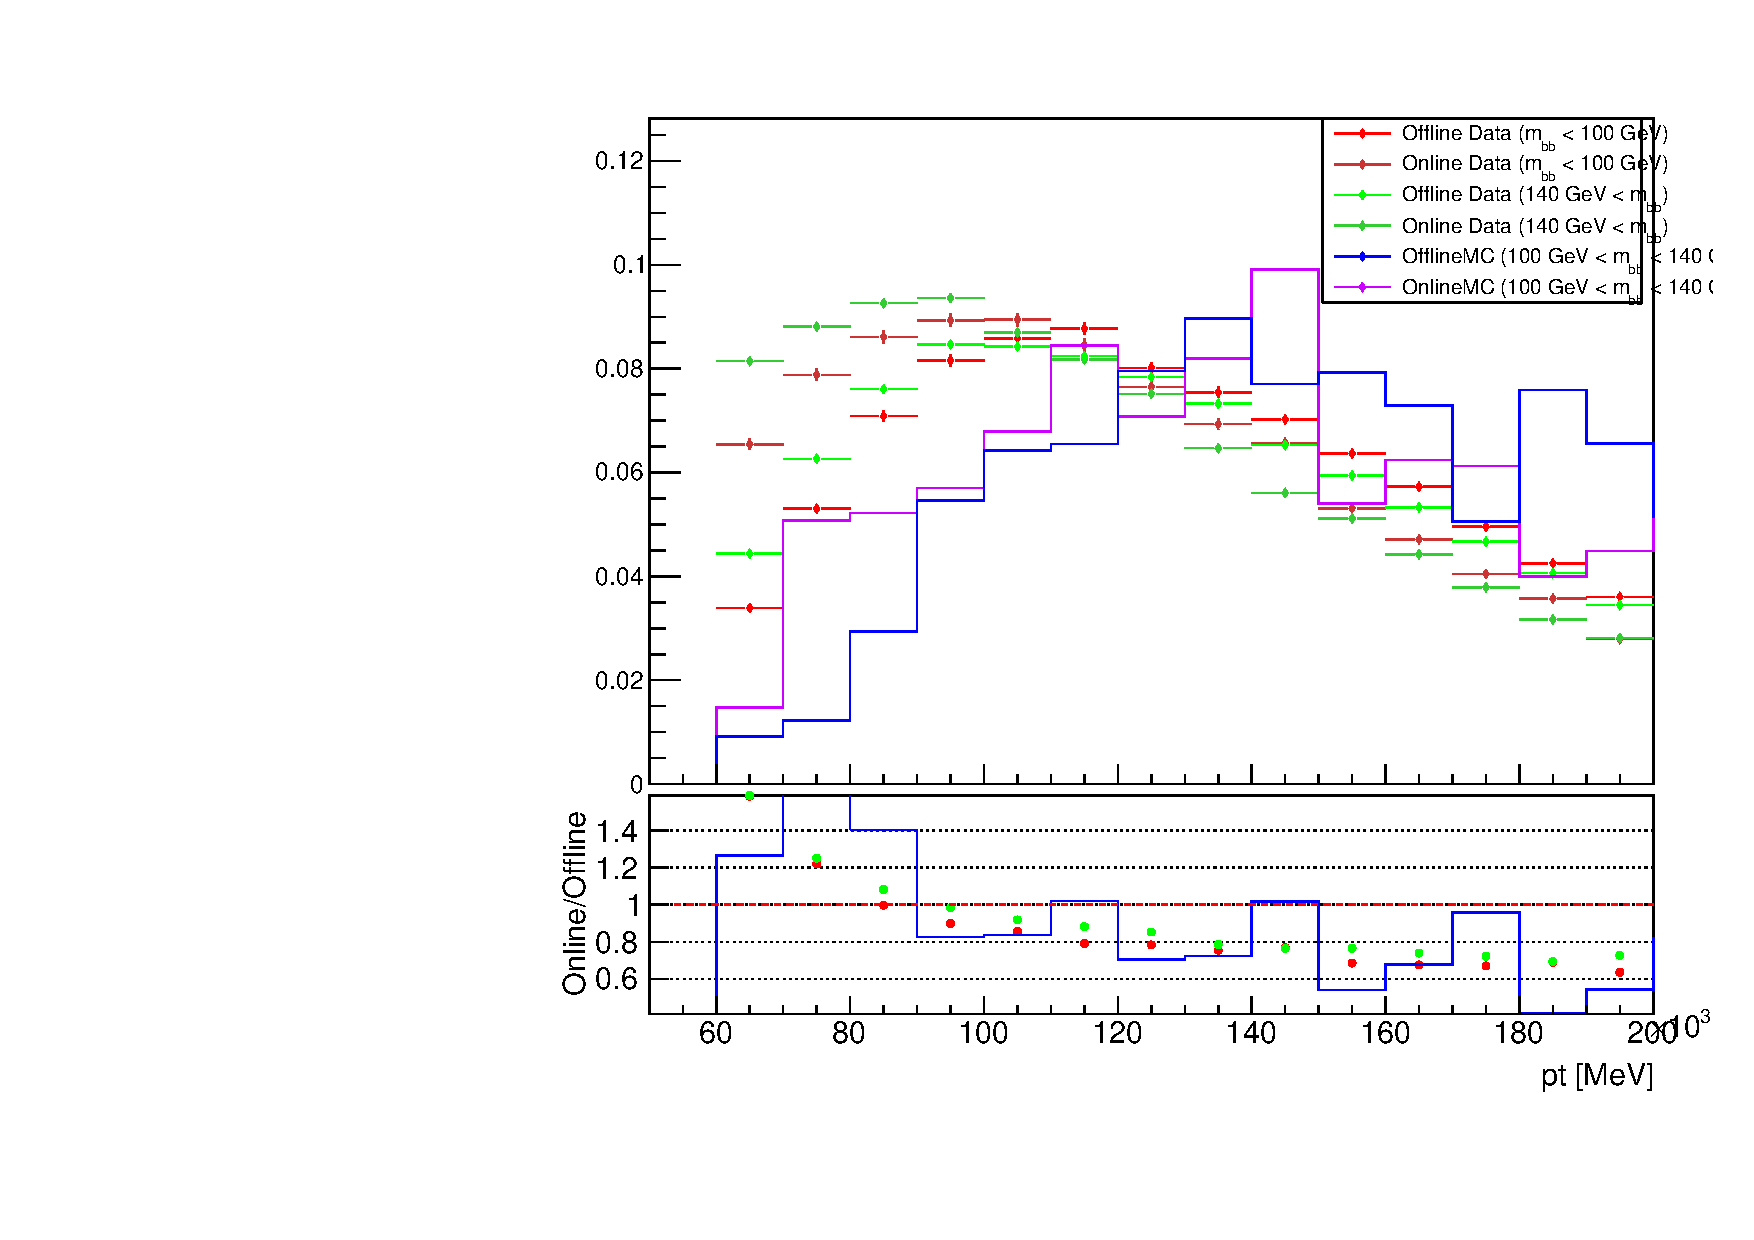
\includegraphics[width=1\linewidth]{pt_lJet1}
				\end{minipage}
				\quad
				\begin{minipage}[h]{0.33\linewidth}
					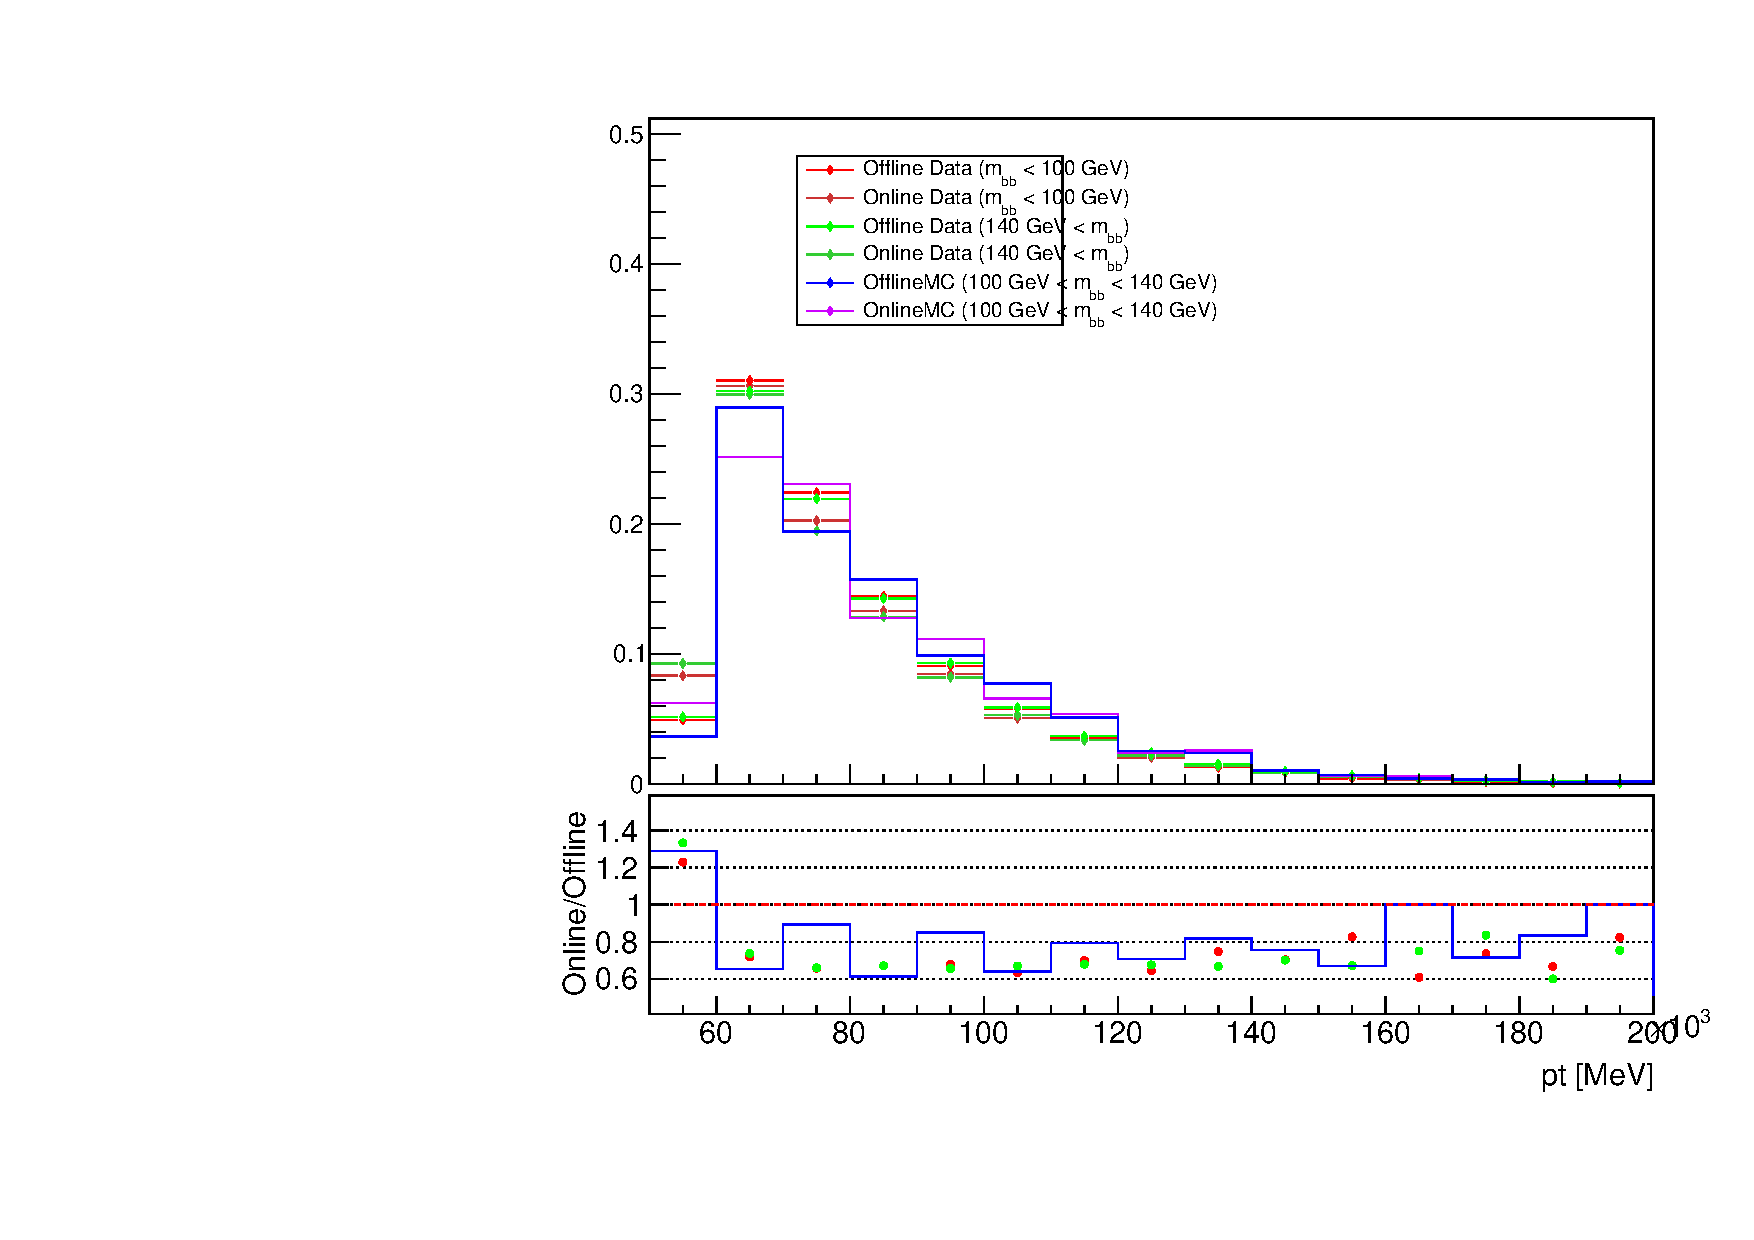
\includegraphics[width=1\linewidth]{pt_lJet2}
				\end{minipage}
				\label{fig:kin:pt2c4j}
			\end{figure}
			
	
			\subsubsection{$\eta$}
				
				\begin{figure}[h]
					\centering
					
					\begin{minipage}[h]{0.33\linewidth}
						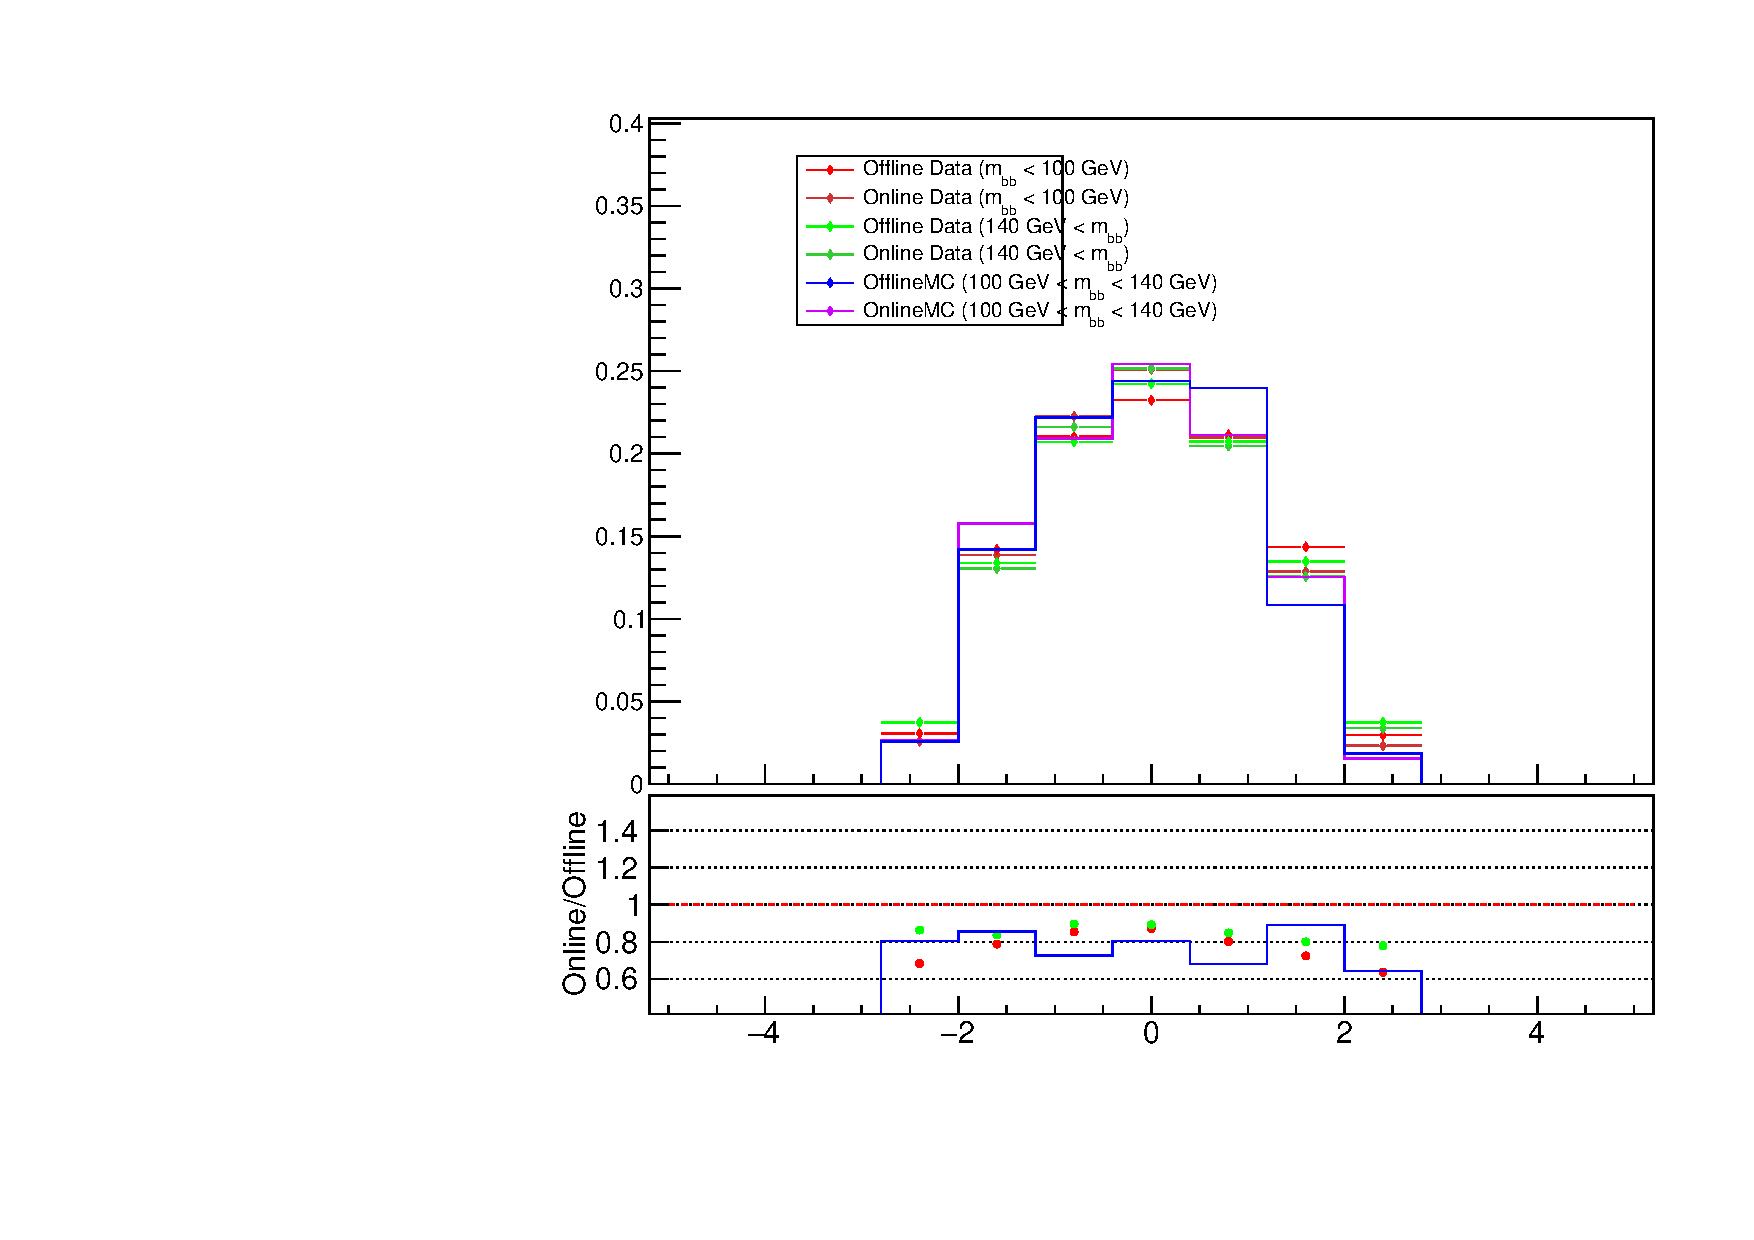
\includegraphics[width=1\linewidth]{eta_bJet1}
					\end{minipage}
					\quad
					\begin{minipage}[h]{0.33\linewidth}
						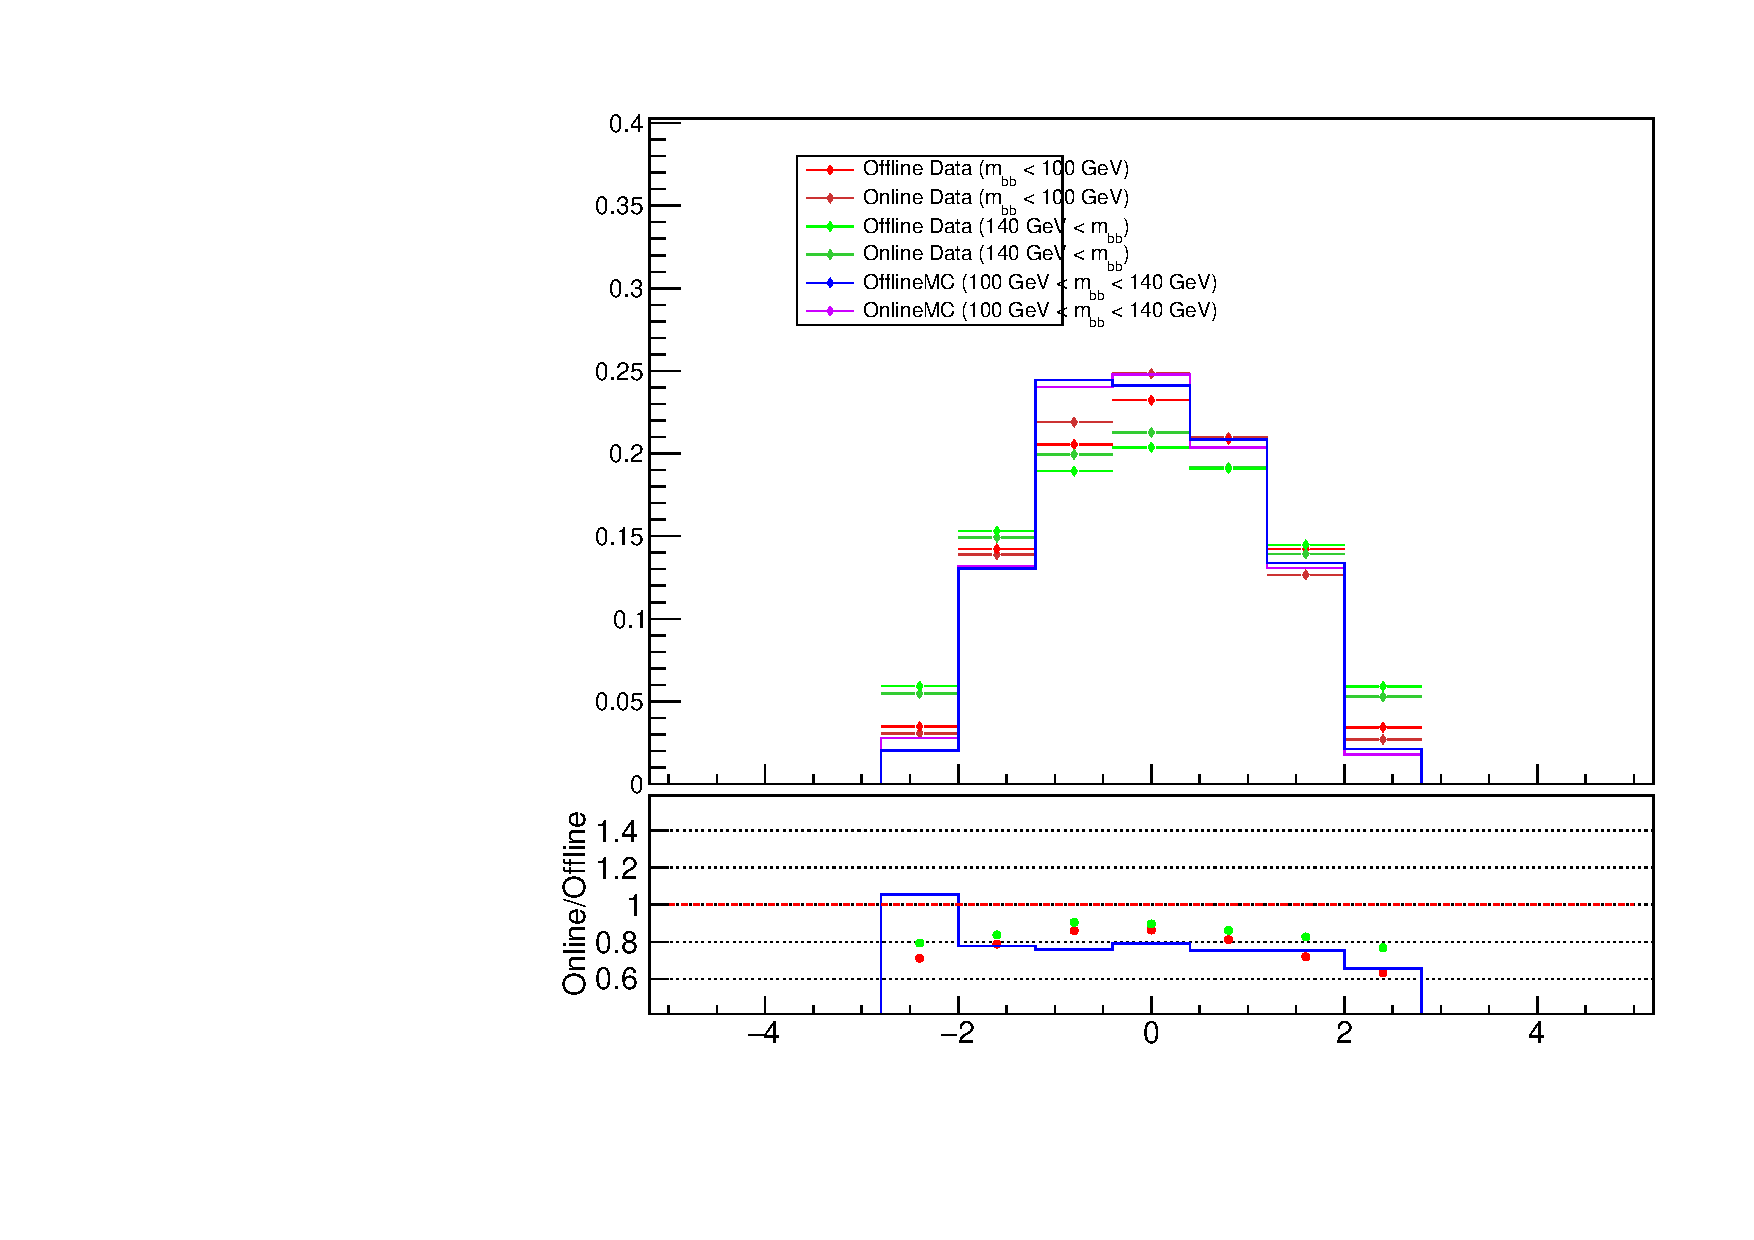
\includegraphics[width=1\linewidth]{eta_bJet2}
					\end{minipage}
					
					\begin{minipage}[h]{0.33\linewidth}
						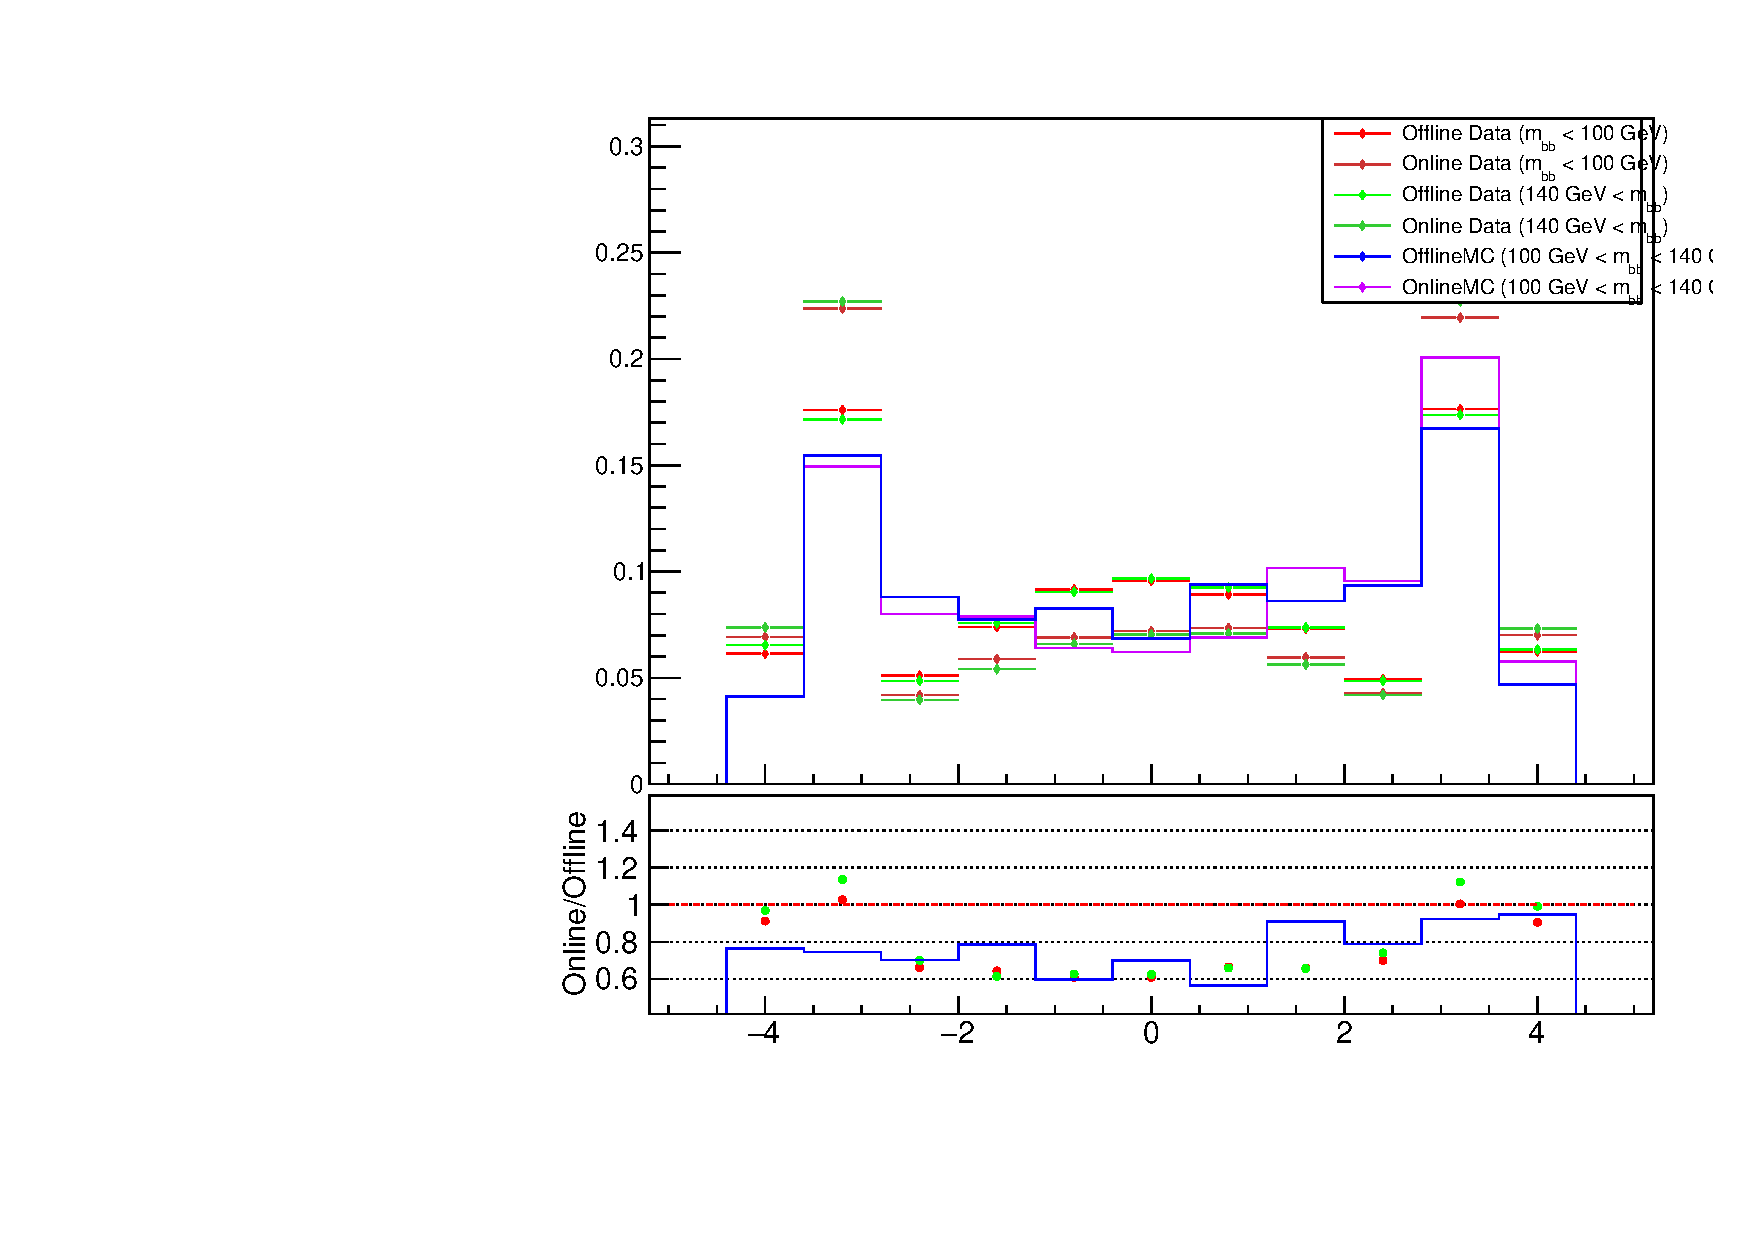
\includegraphics[width=1\linewidth]{eta_lJet1}
					\end{minipage}
					\quad
					\begin{minipage}[h]{0.33\linewidth}
						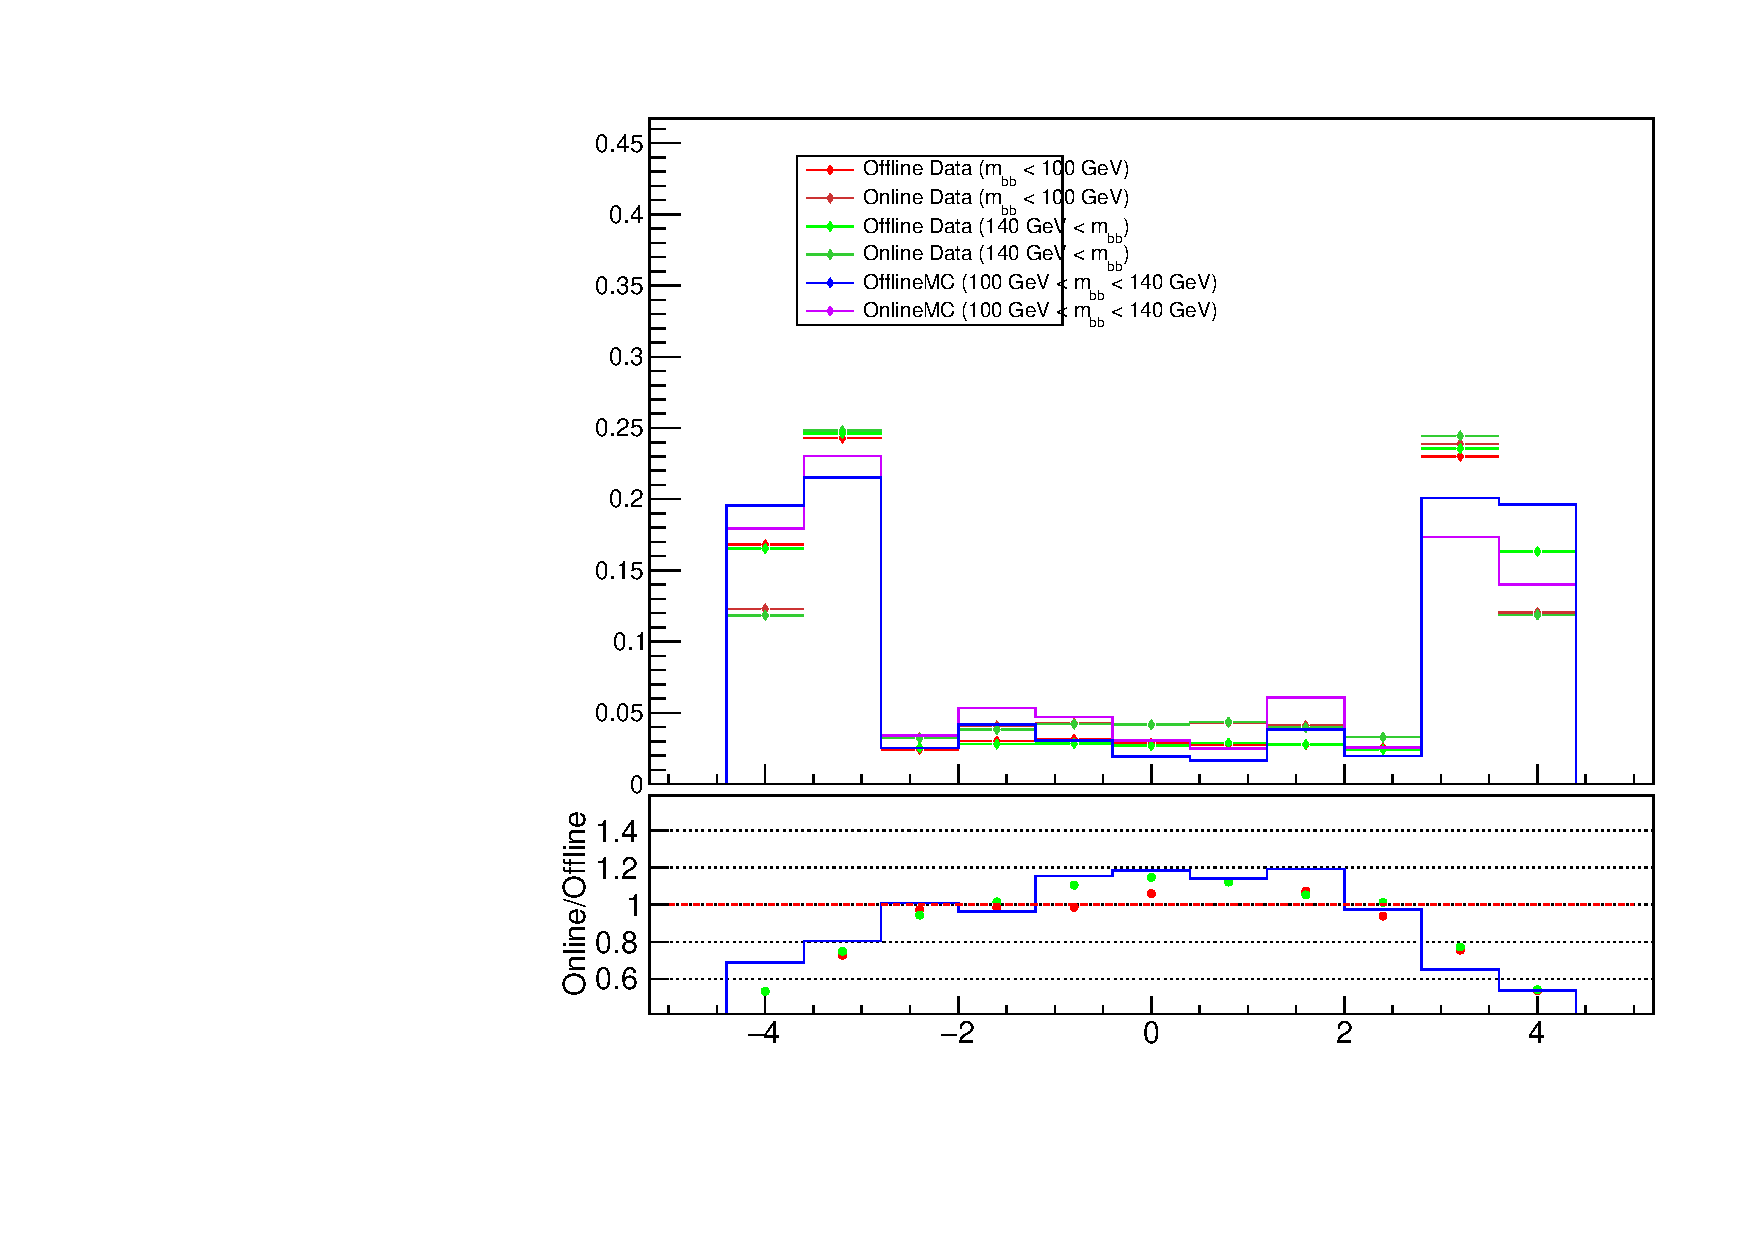
\includegraphics[width=1\linewidth]{eta_lJet2}
					\end{minipage}
					\label{fig:kin:eta2c4j}
				\end{figure}
				
		\subsubsection{$\phi$}
		
		\begin{figure}[h]
			\centering
			
			\begin{minipage}[h]{0.33\linewidth}
				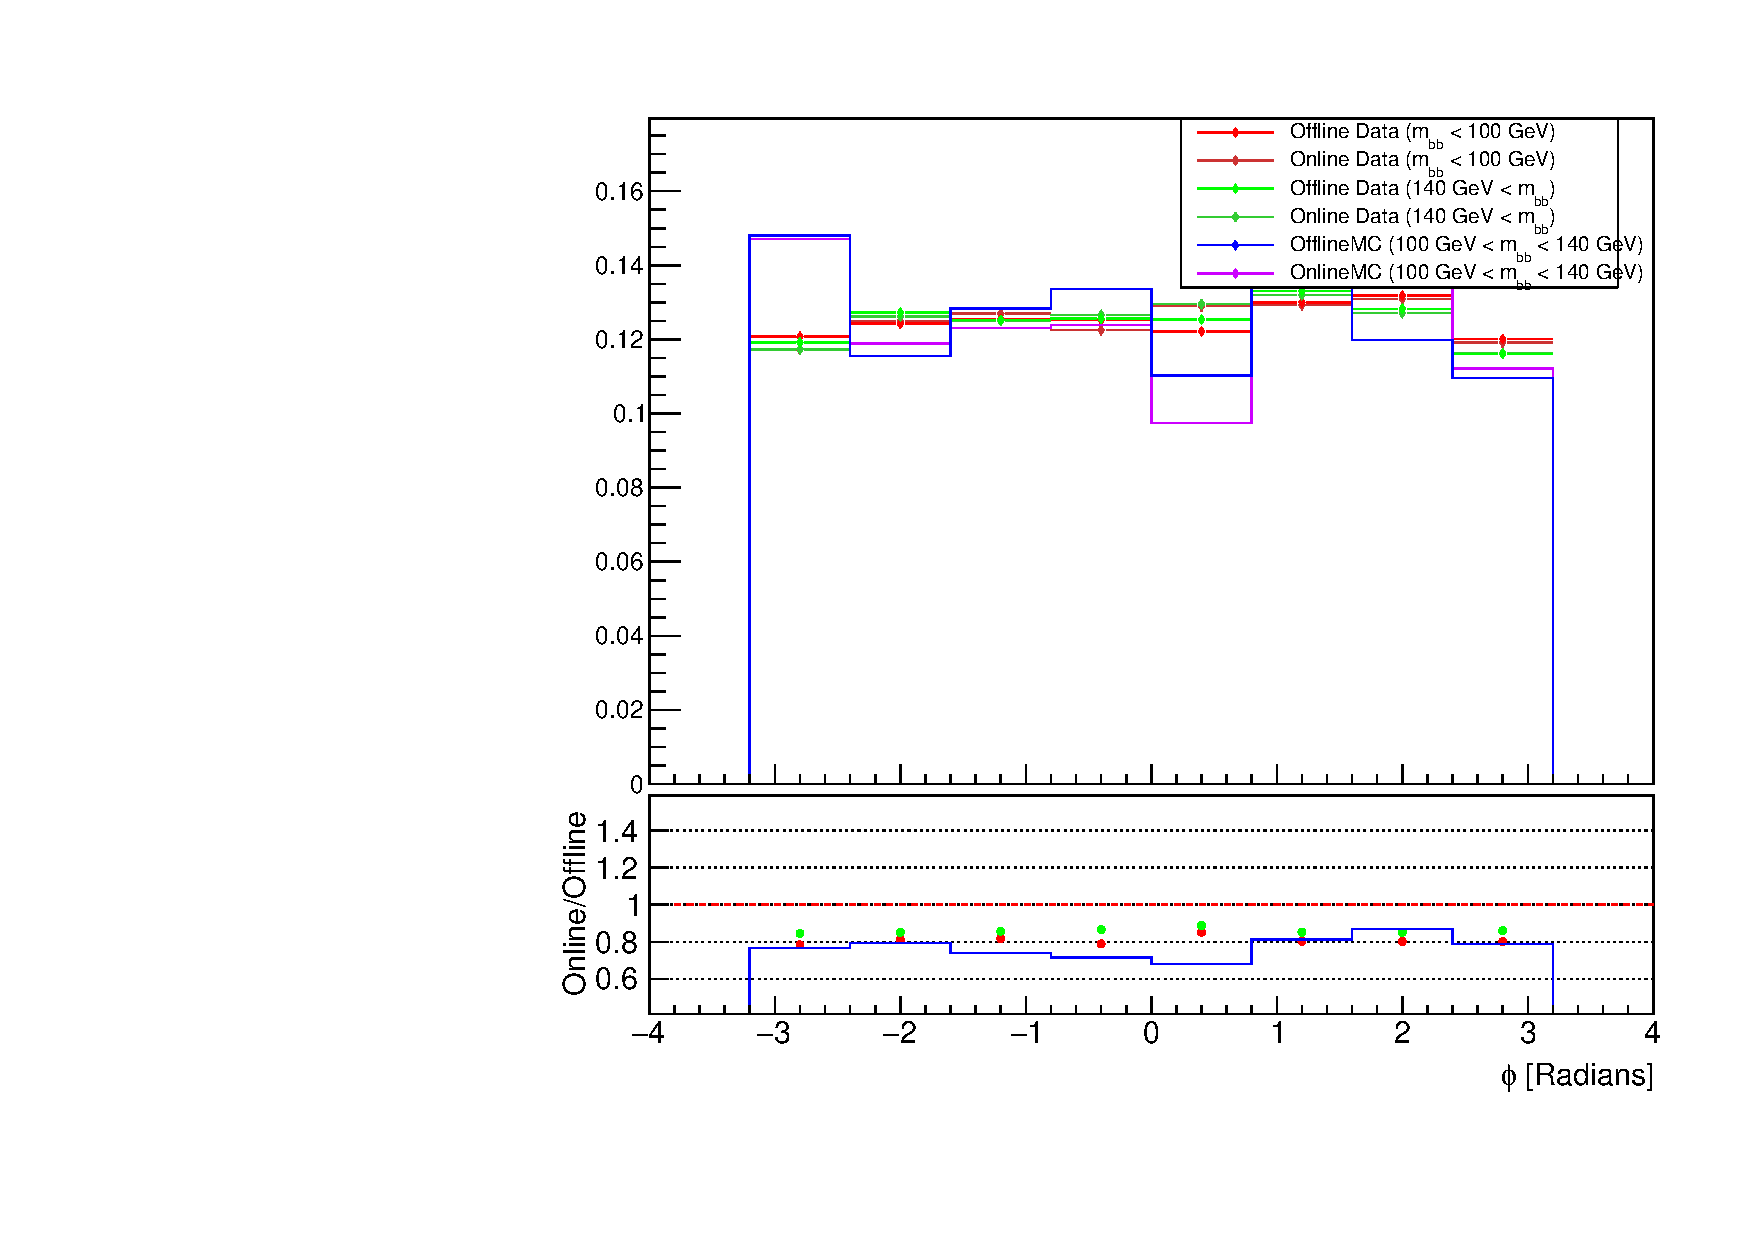
\includegraphics[width=1\linewidth]{phi_bJet1}
			\end{minipage}
			\quad
			\begin{minipage}[h]{0.33\linewidth}
				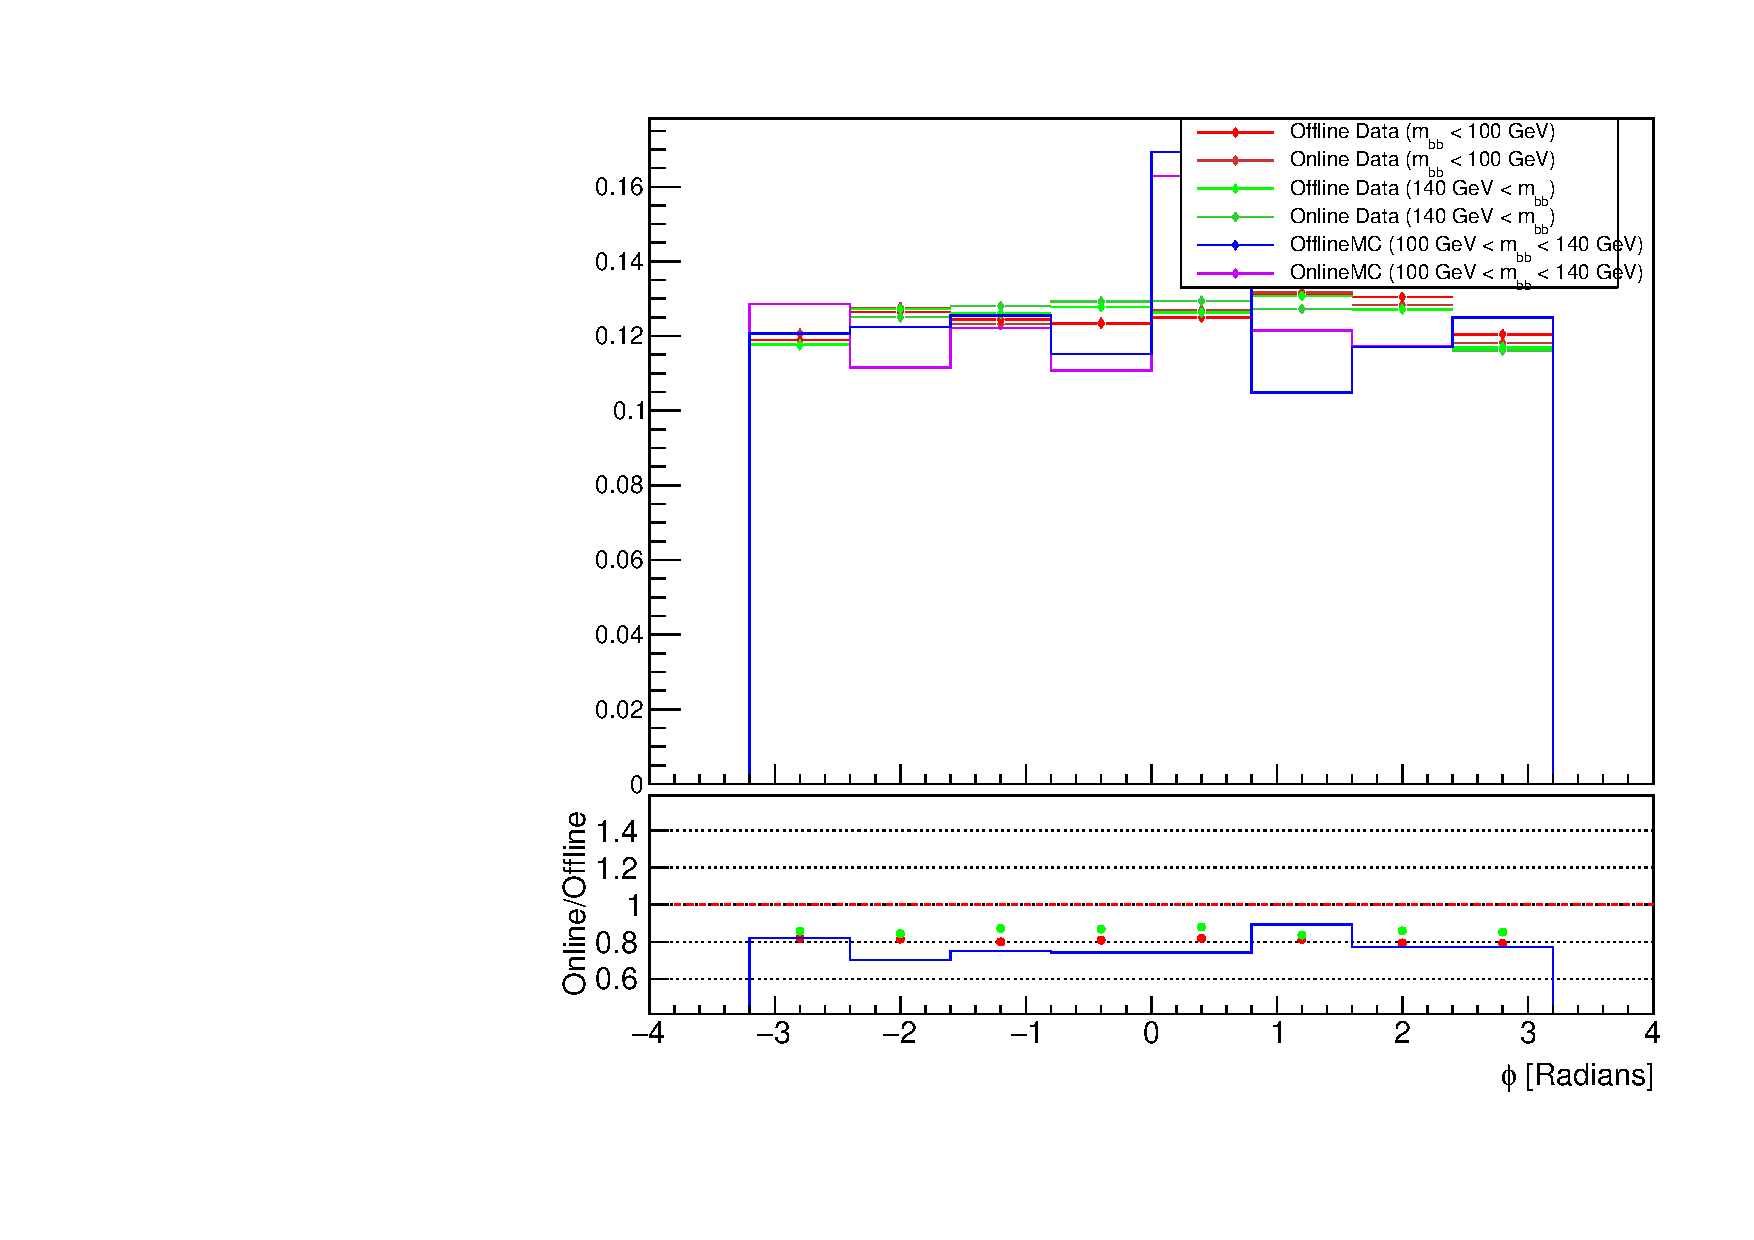
\includegraphics[width=1\linewidth]{phi_bJet2}
			\end{minipage}
			
			\begin{minipage}[h]{0.33\linewidth}
				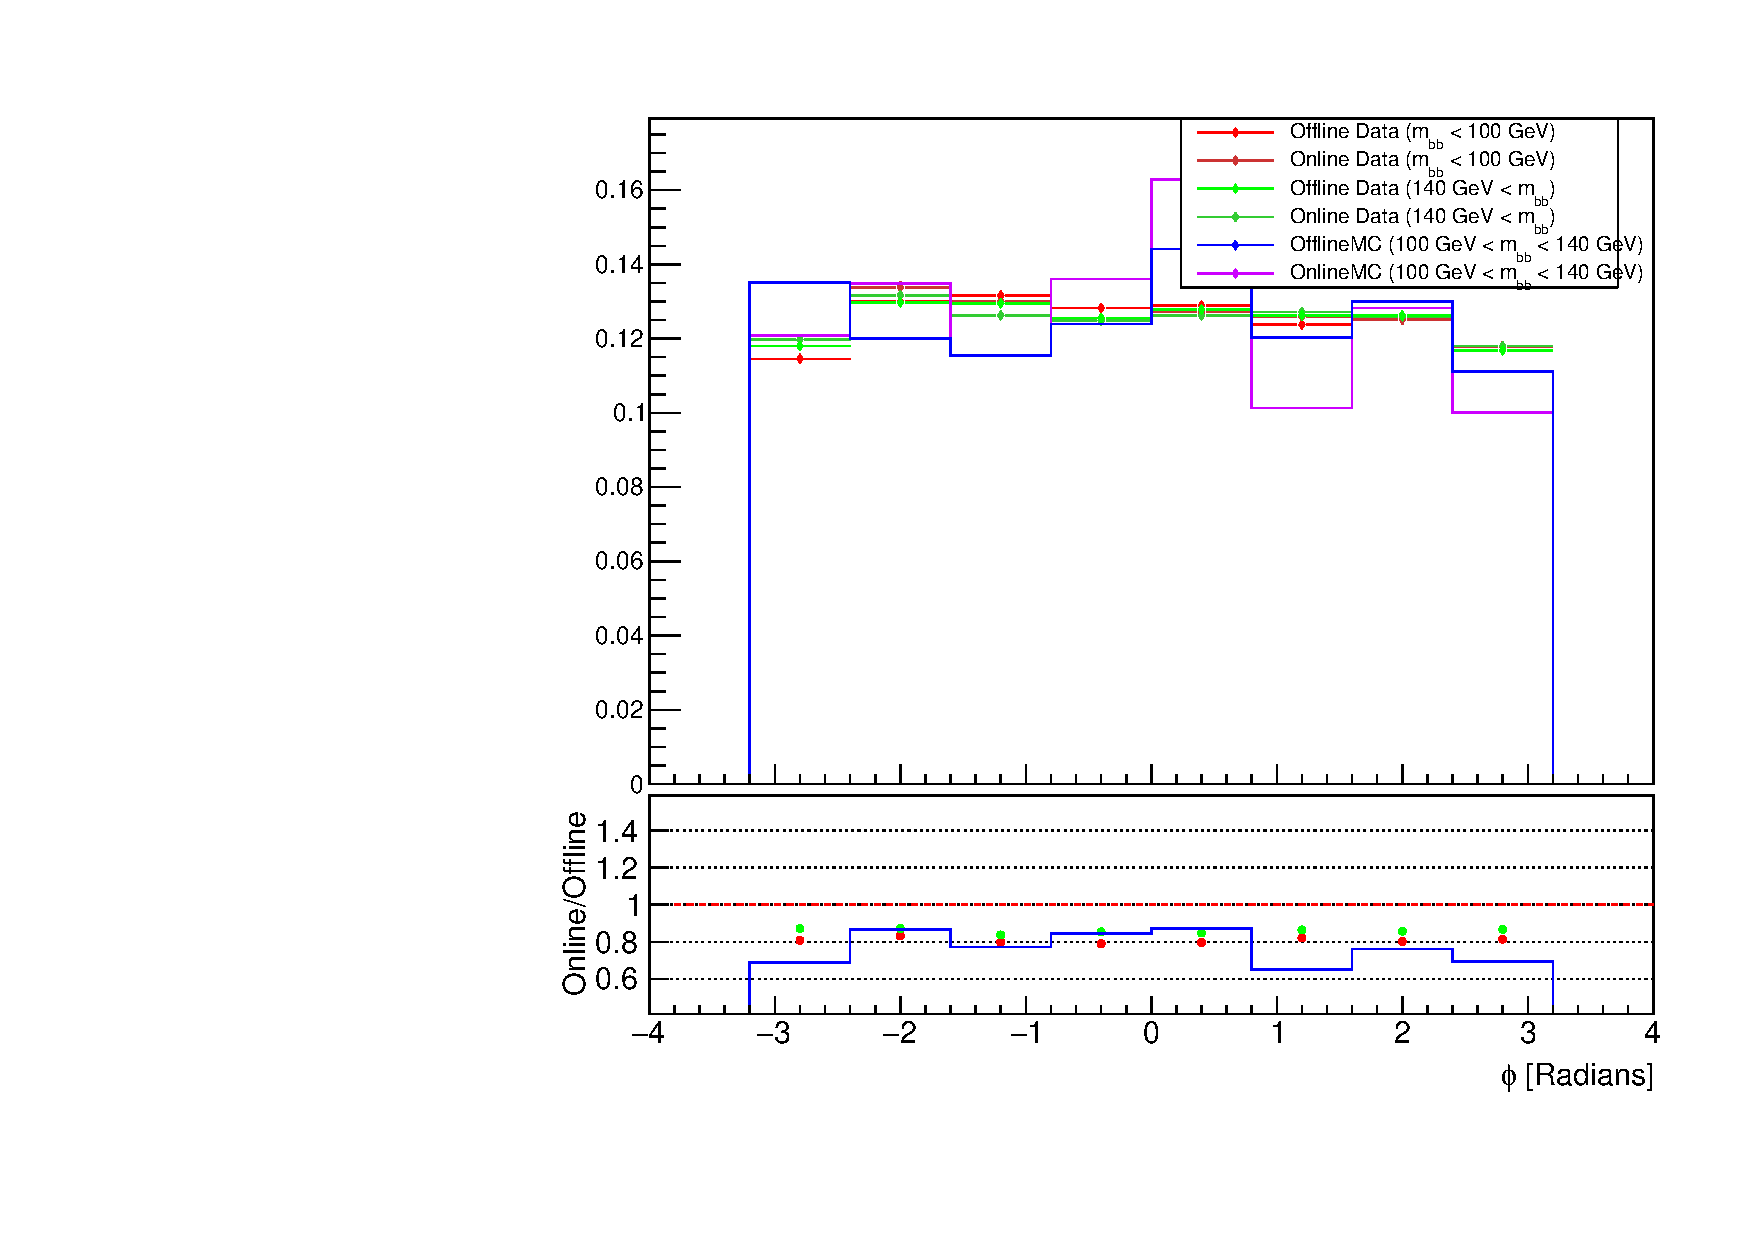
\includegraphics[width=1\linewidth]{phi_lJet1}
			\end{minipage}
			\quad
			\begin{minipage}[h]{0.33\linewidth}
				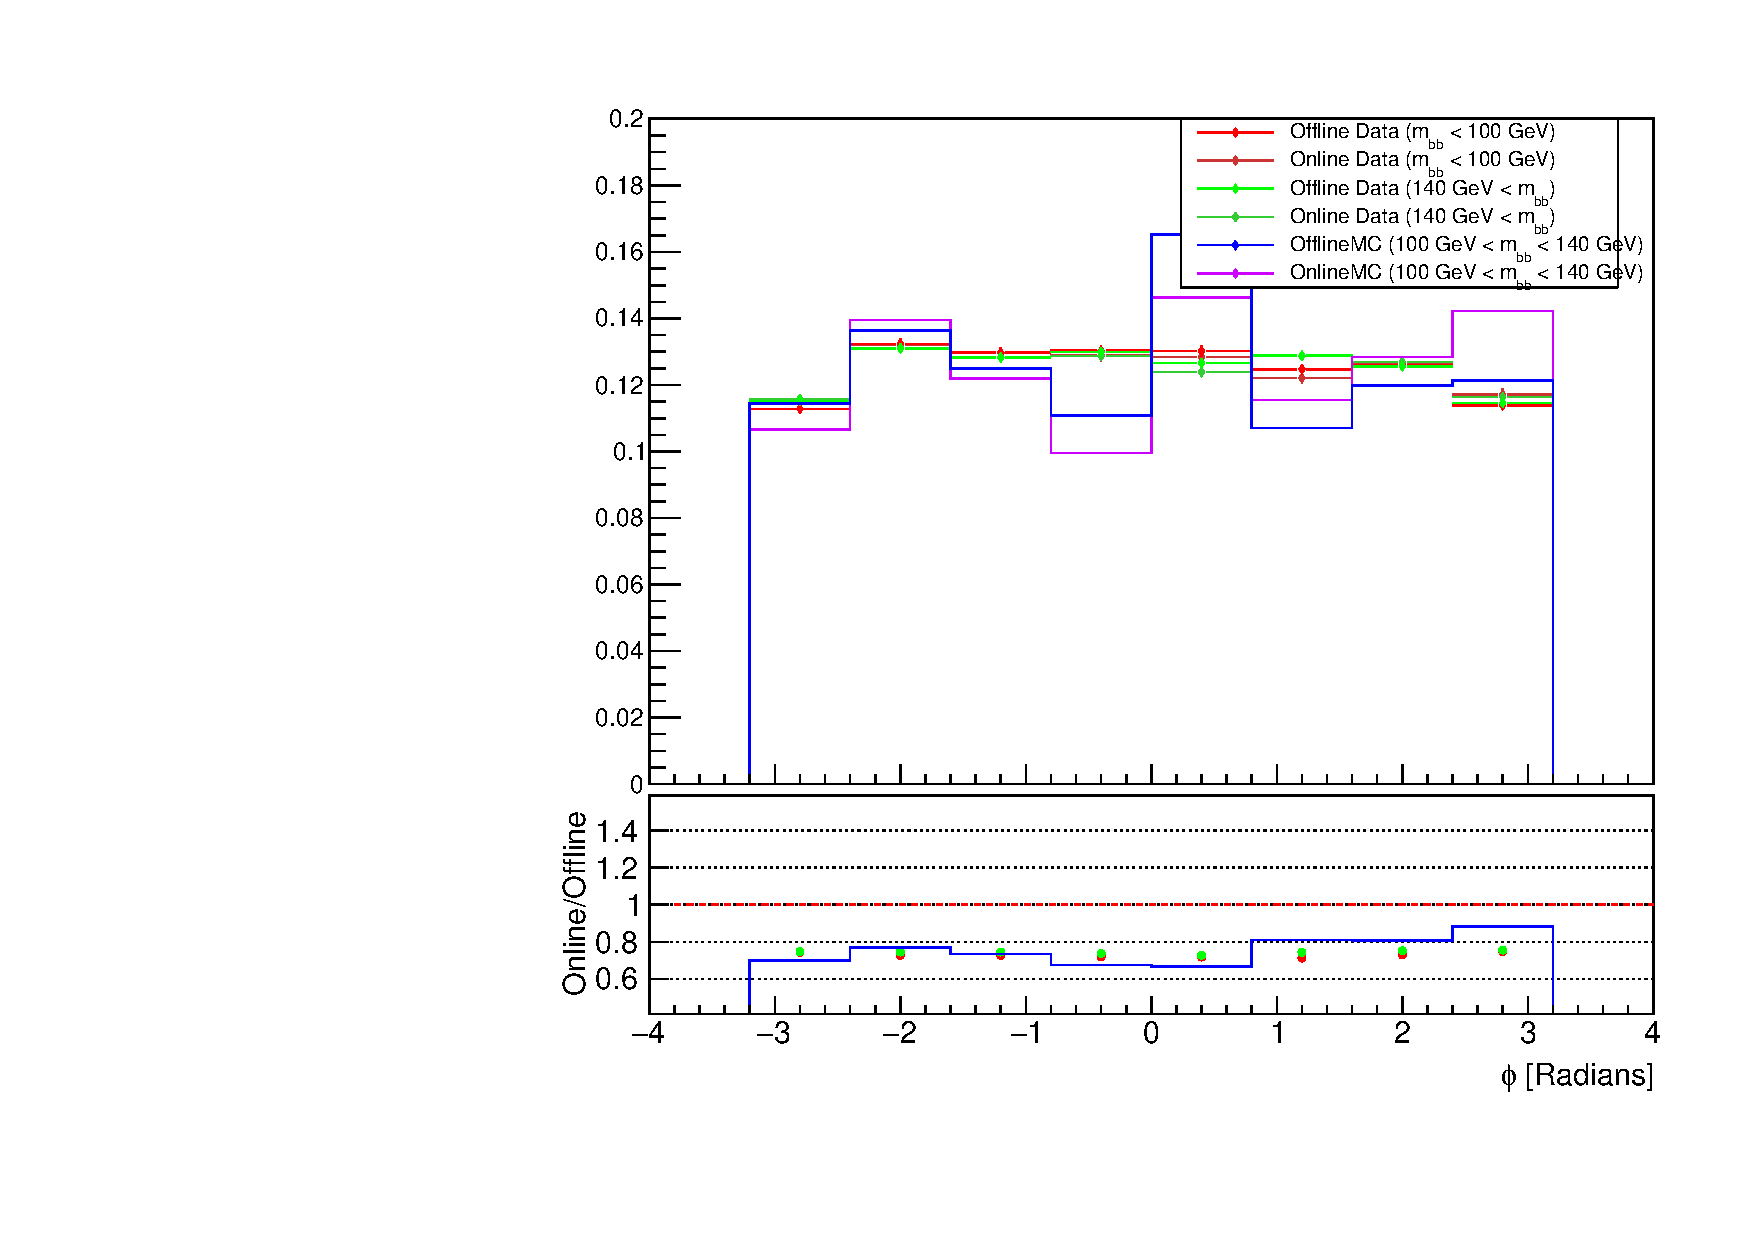
\includegraphics[width=1\linewidth]{phi_lJet2}
			\end{minipage}
			\label{fig:kin:phi2c4j}
		\end{figure}
		
				\subsubsection{M}
				
				\begin{figure}[h]
					\centering
					
					\begin{minipage}[h]{0.33\linewidth}
						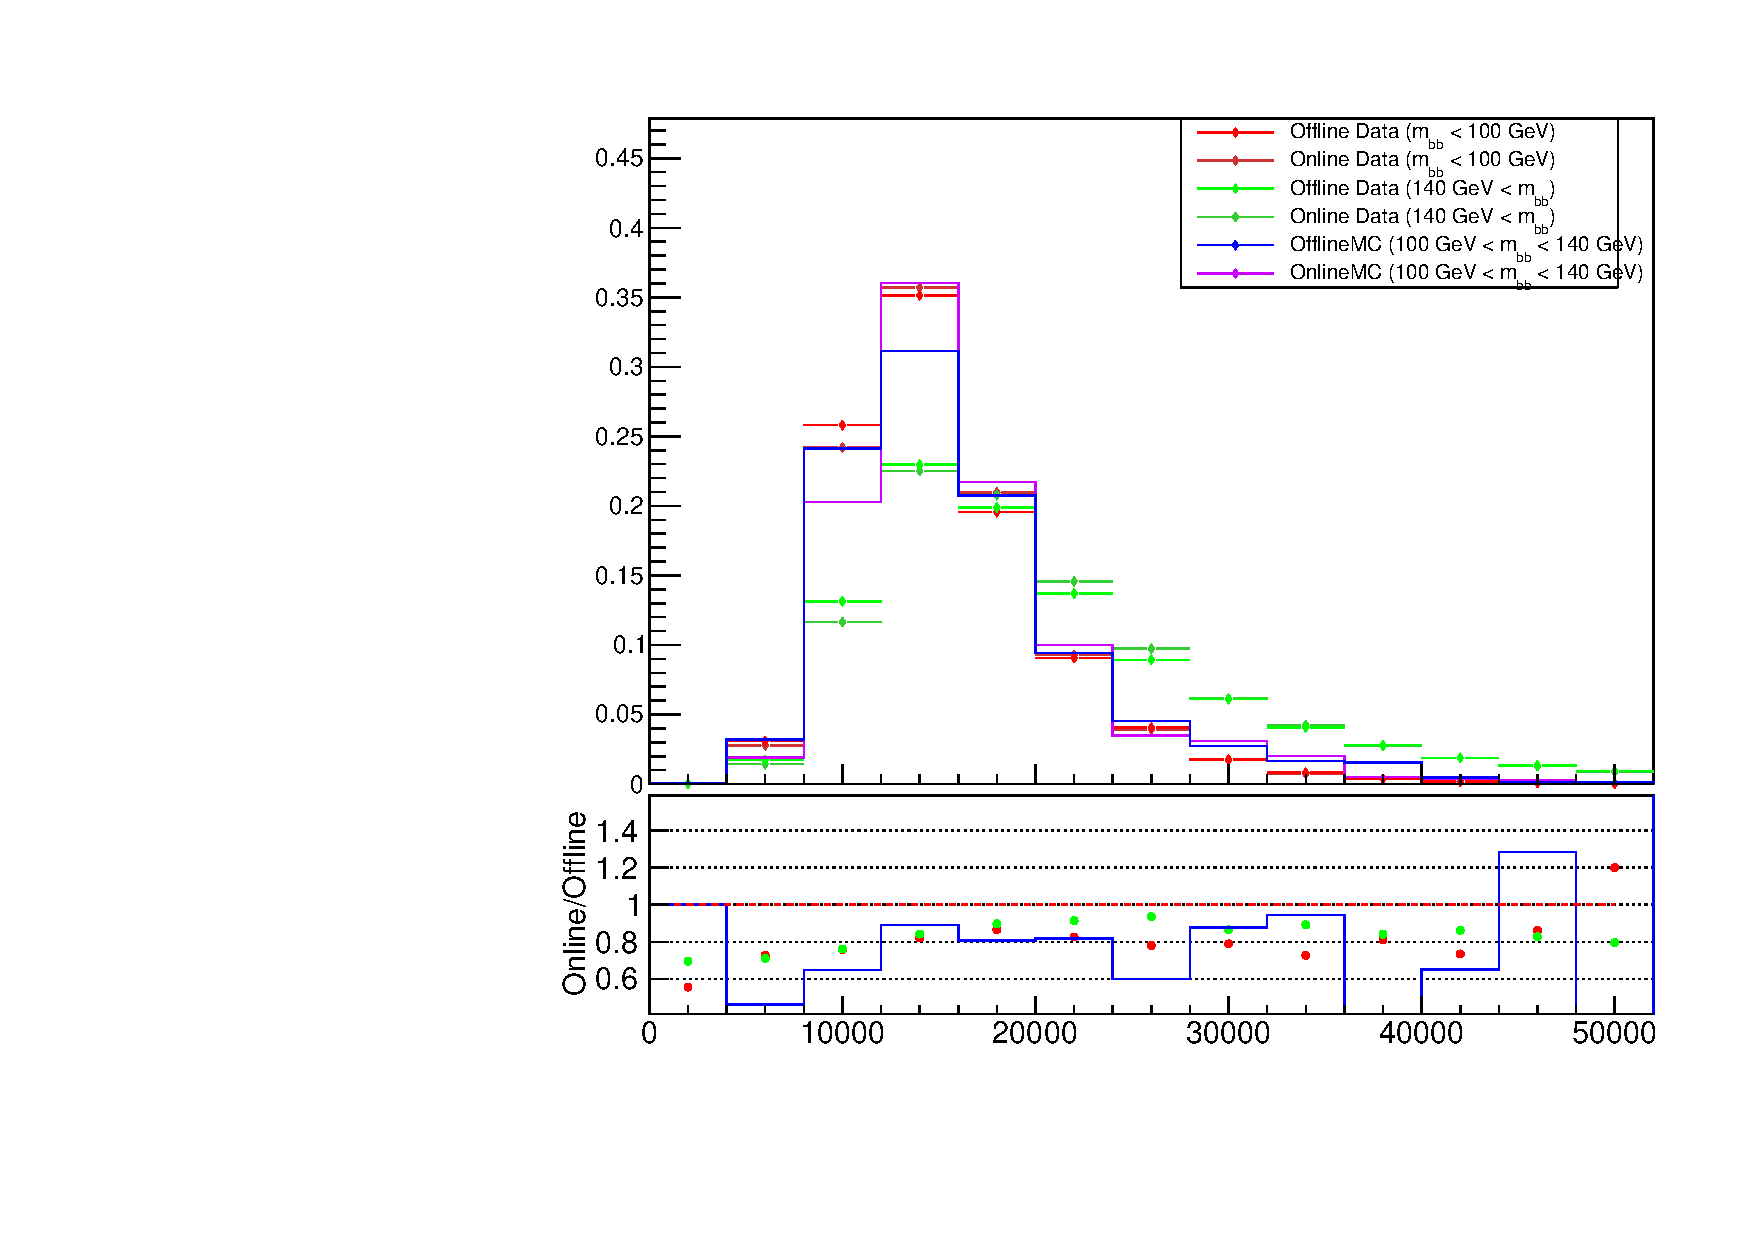
\includegraphics[width=1\linewidth]{m_bJet1}
					\end{minipage}
					\quad
					\begin{minipage}[h]{0.33\linewidth}
						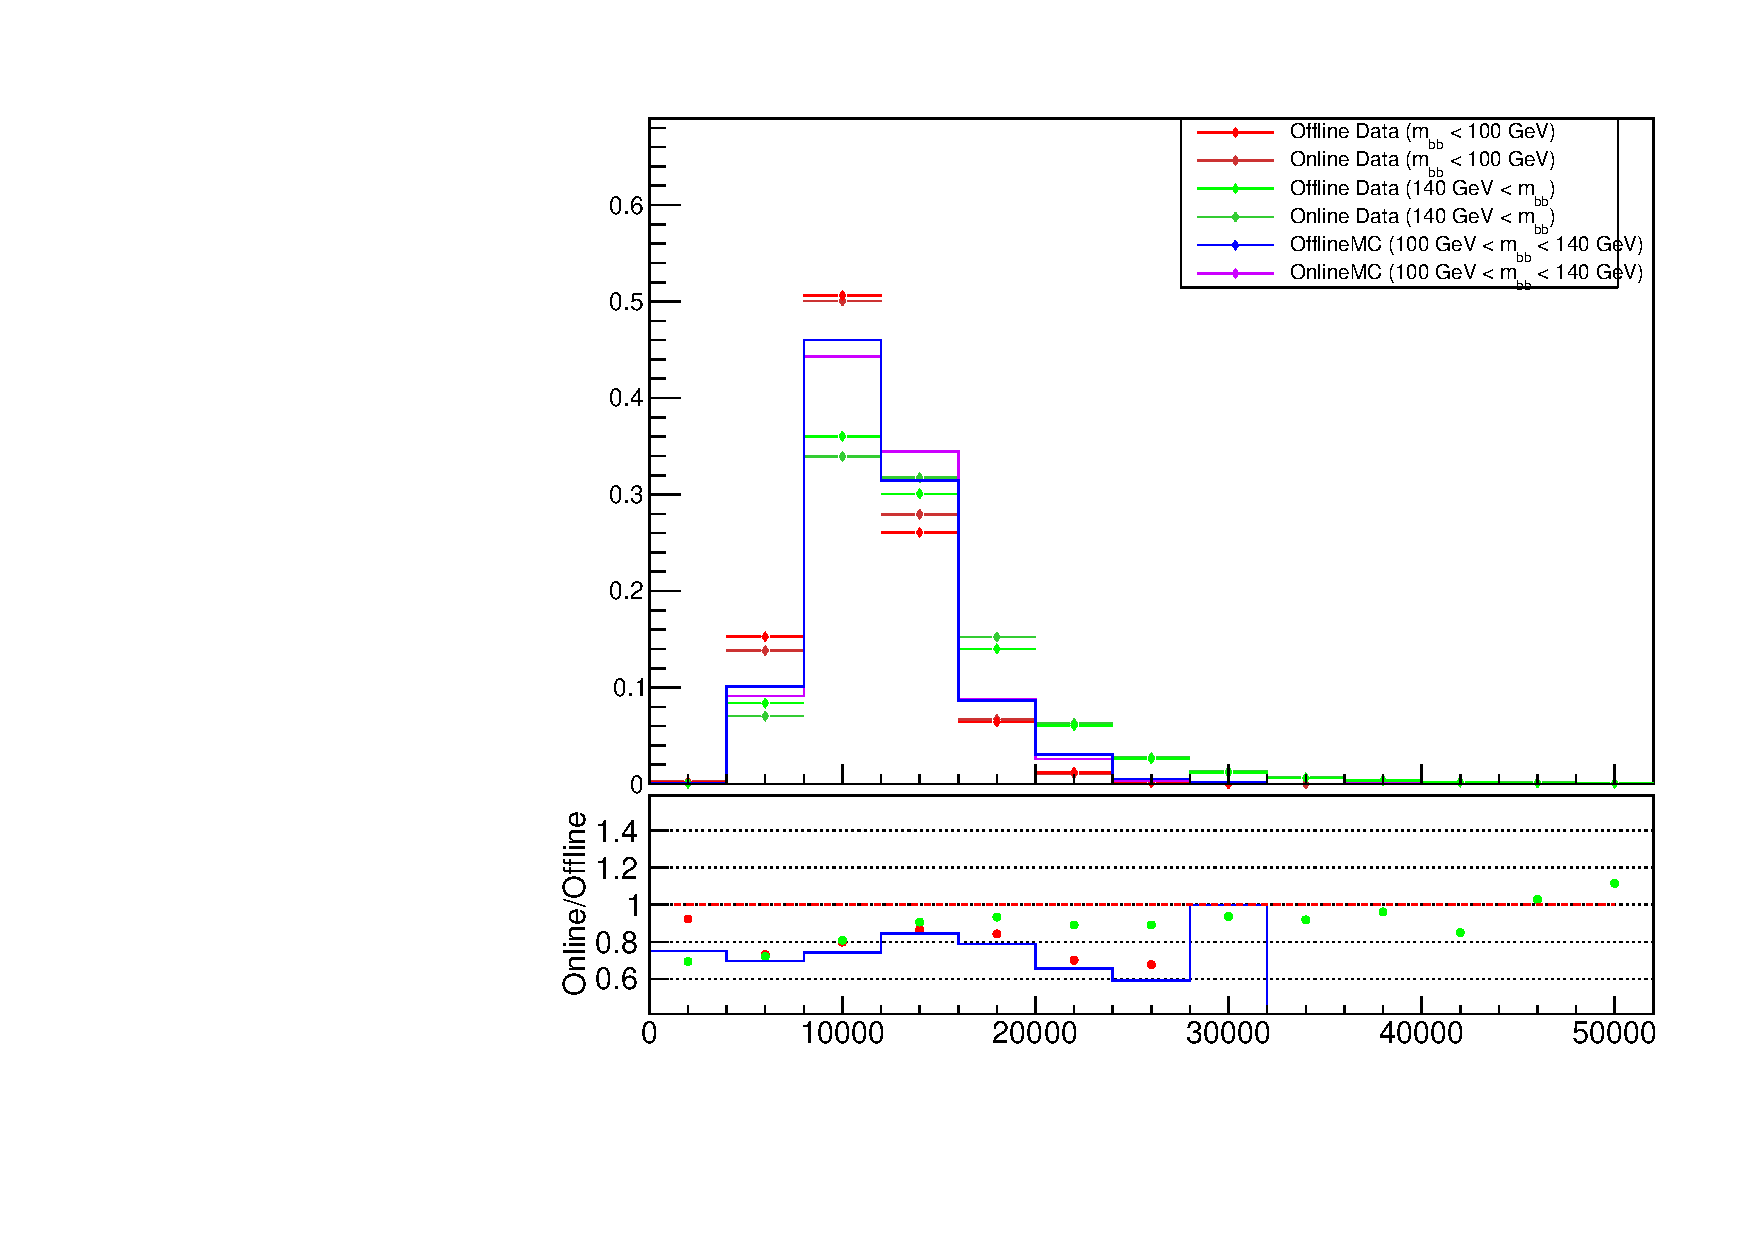
\includegraphics[width=1\linewidth]{m_bJet2}
					\end{minipage}
					
					\begin{minipage}[h]{0.33\linewidth}
						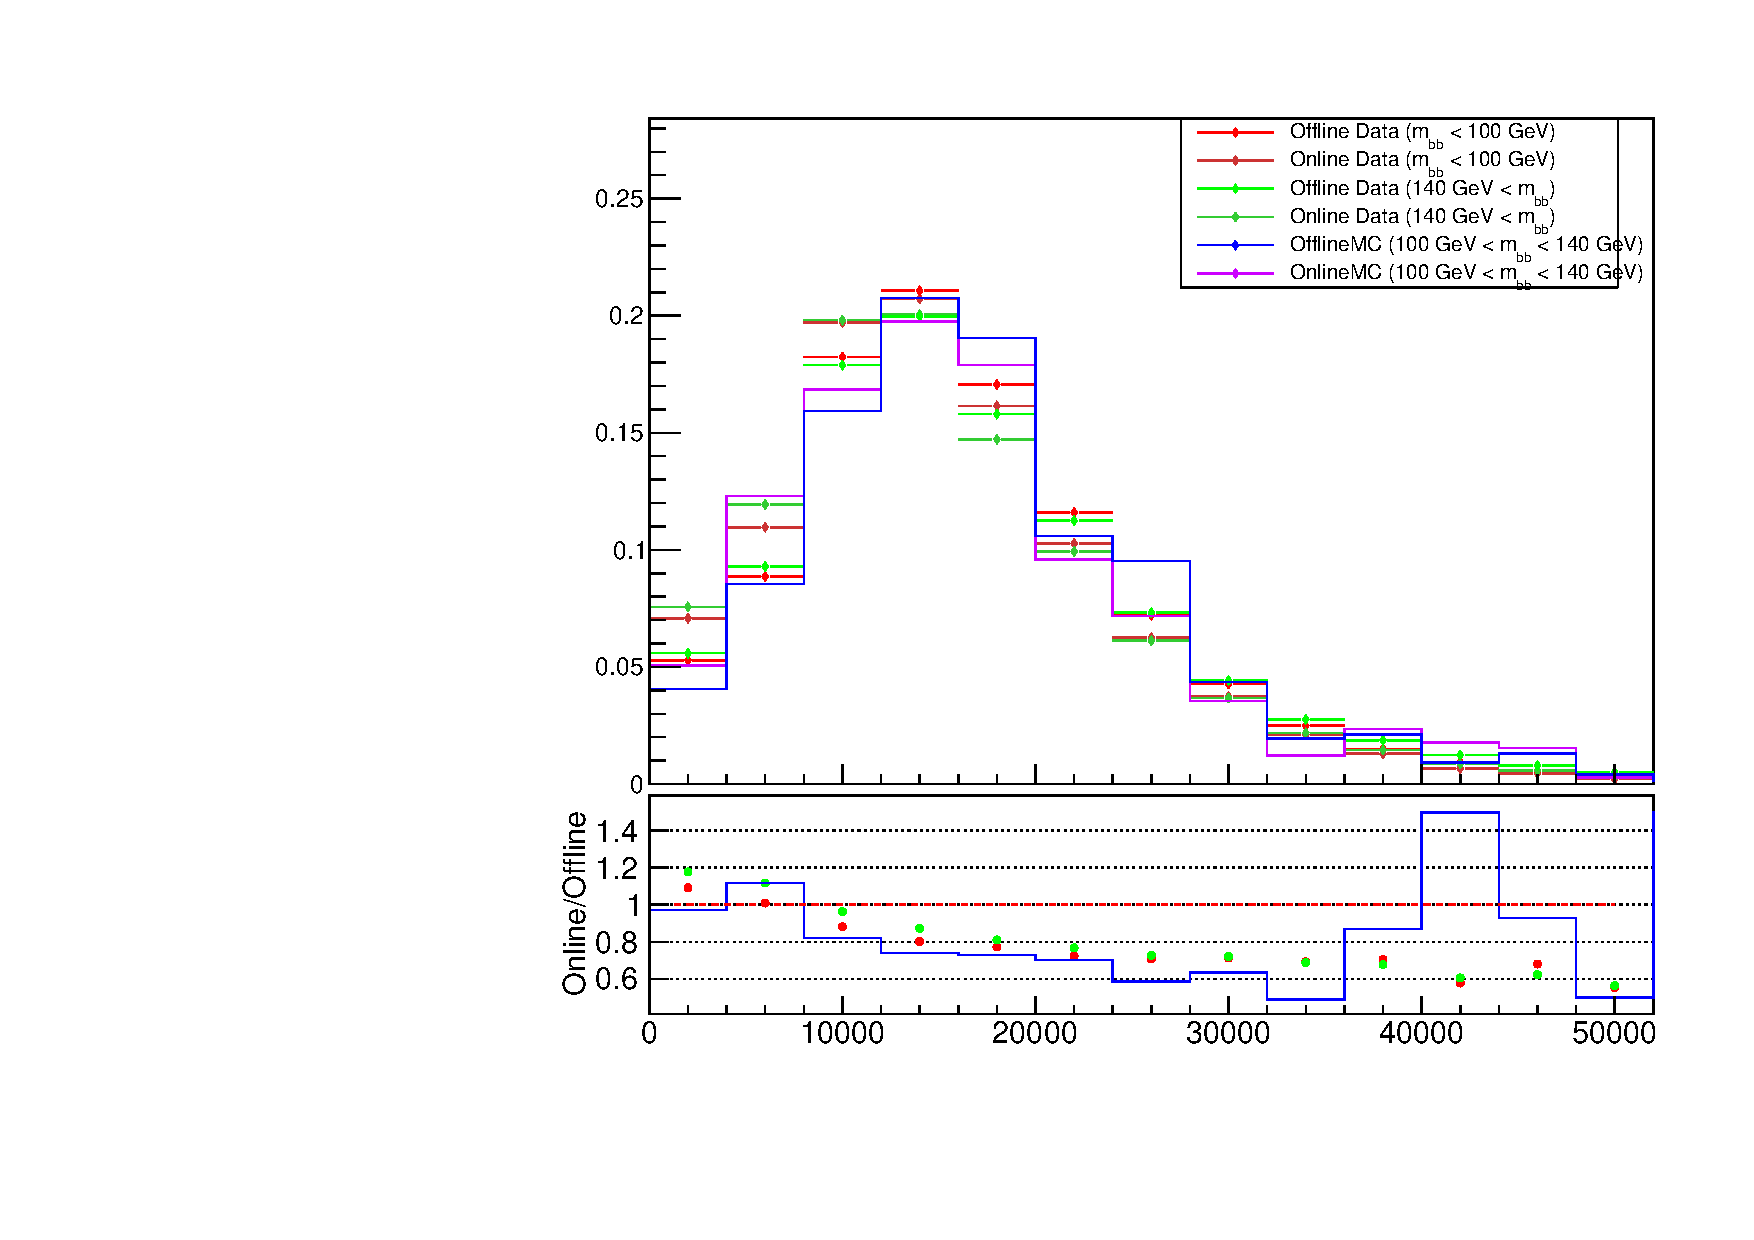
\includegraphics[width=1\linewidth]{m_lJet1}
					\end{minipage}
					\quad
					\begin{minipage}[h]{0.33\linewidth}
						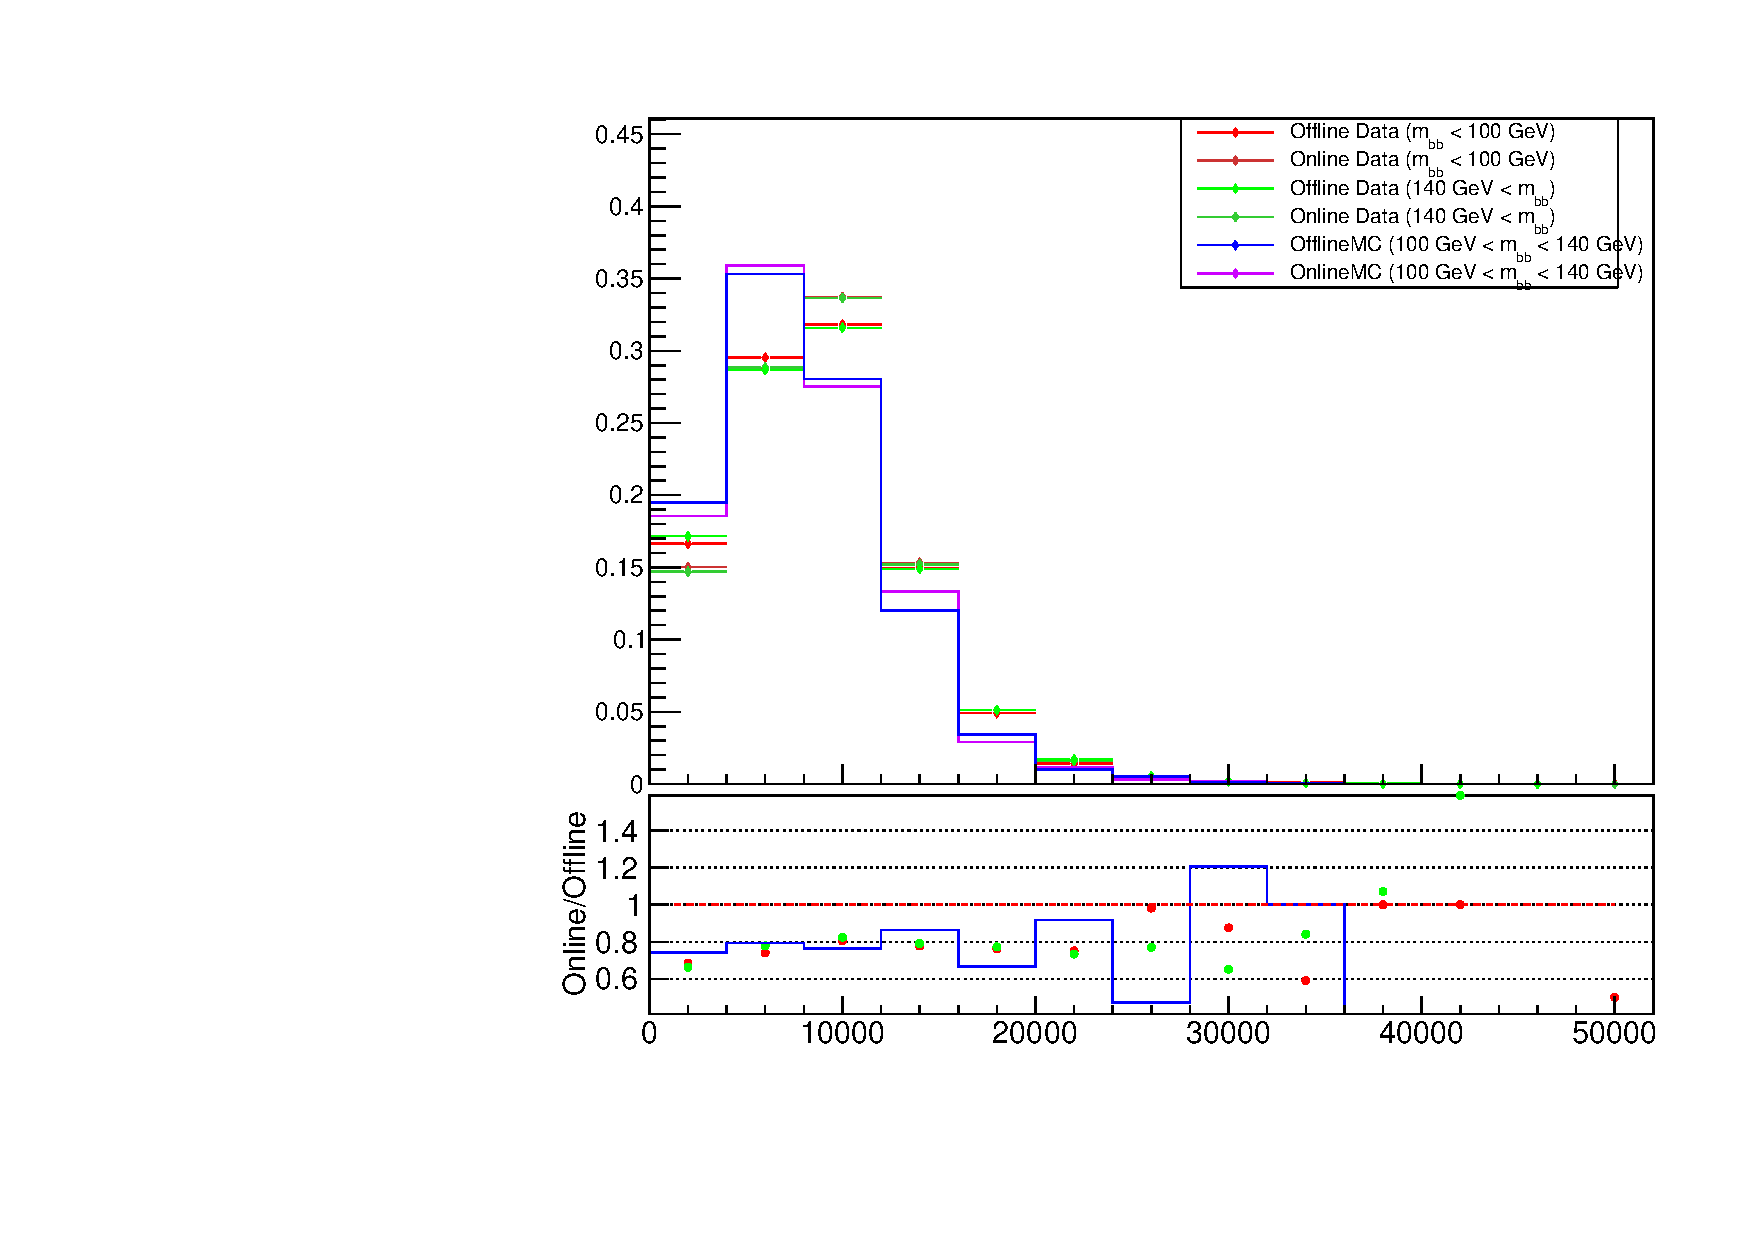
\includegraphics[width=1\linewidth]{m_lJet2}
					\end{minipage}`
					\label{fig:kin:m2c4j}
				\end{figure}
		


\section{BDT Input Variables}

	\begin{itemize}
		\item $M_{jj}$
		\item \pt$_{jj}$
		\item $\cos \theta$
		\item $\Delta\eta_{jj}$
		\item $Max(\eta)$
		\item $\eta*$
		\item $min\Delta R(j_1)$
		\item $min\Delta R(j_1)$
		\item \pt balance
		\item $N_{TRK}(j_1) PV500$ ?
		\item $N_{TRK}(j_) PV500$ ?
	\end{itemize}
	
		\begin{figure}[h]
			\centering1
			\begin{minipage}[h]{0.45\linewidth}
				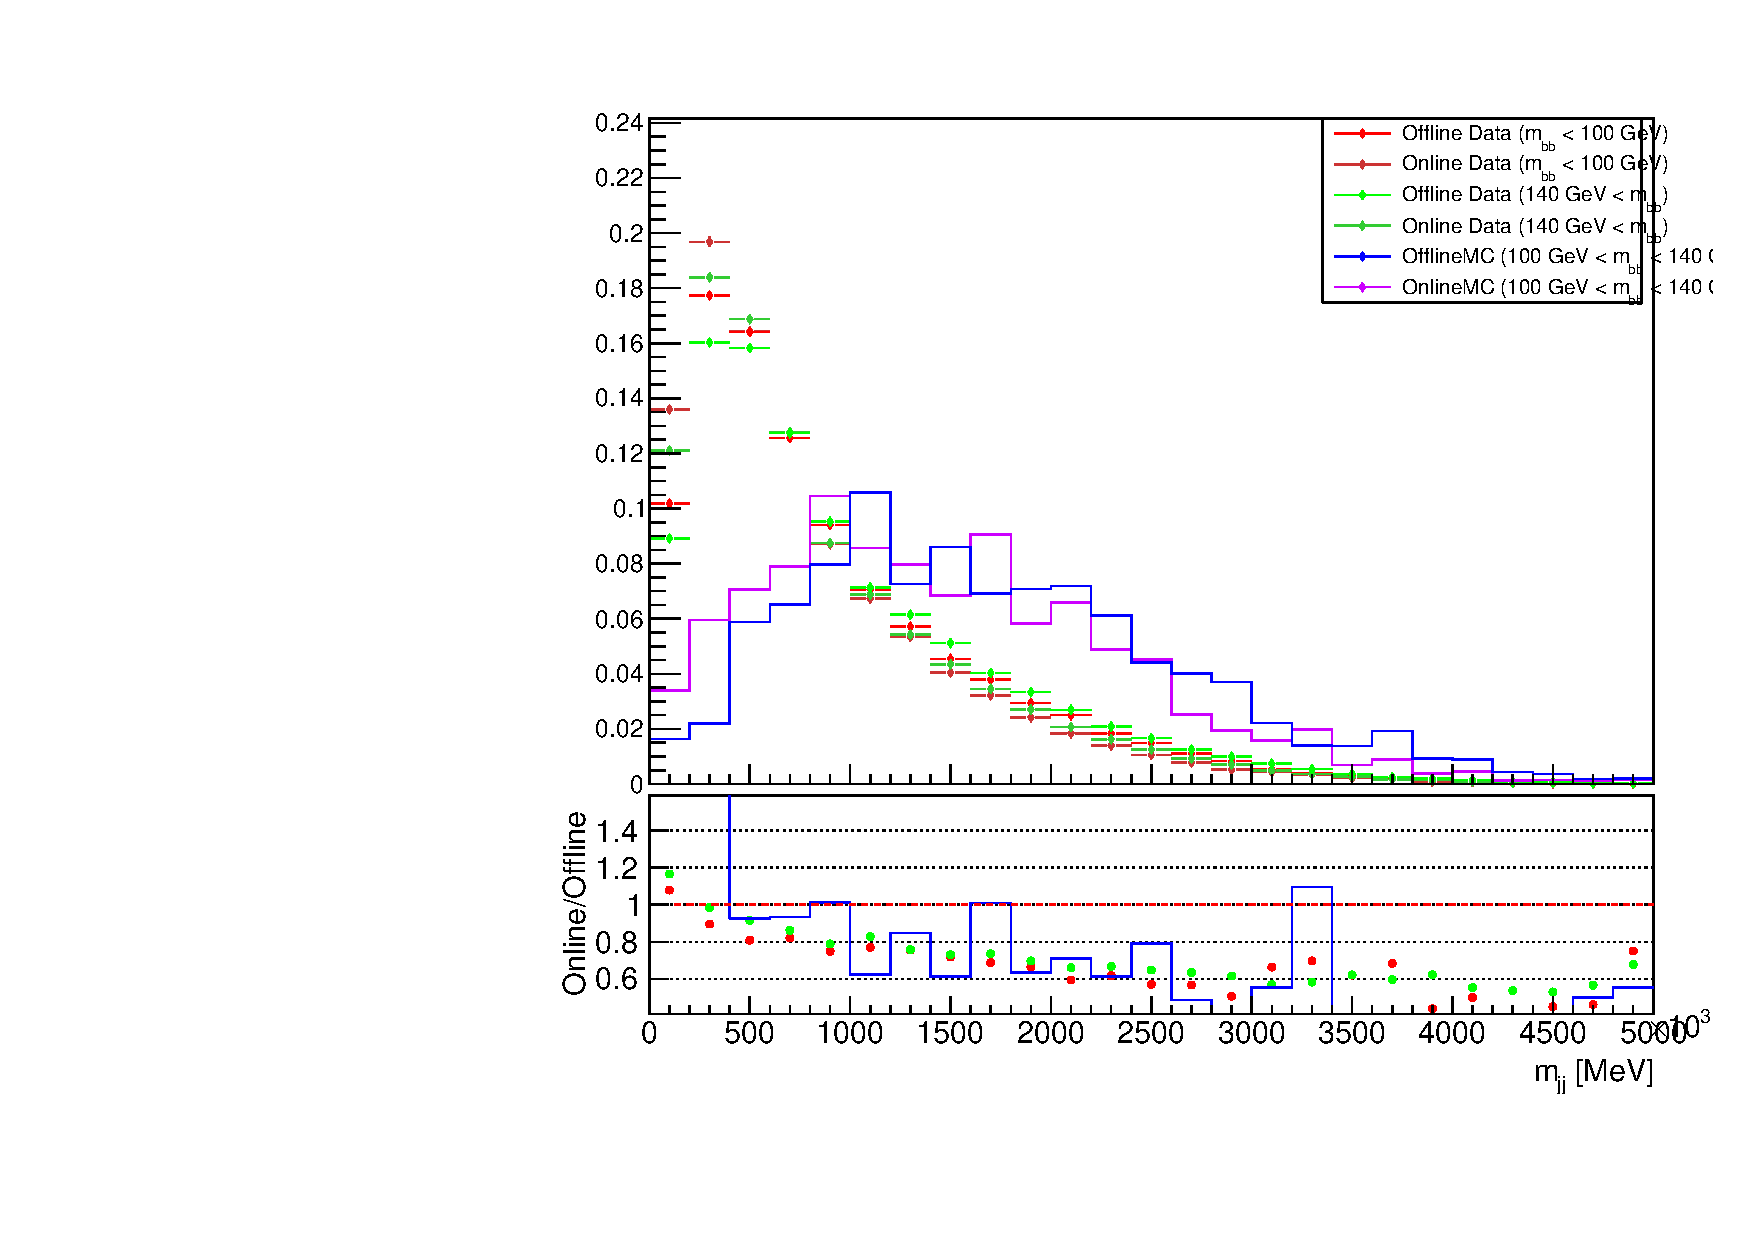
\includegraphics[width=1\linewidth]{mjj}
				\caption{}
				\label{fig:bdtmjj}
			\end{minipage}
			\quad
			\begin{minipage}[h]{0.45\linewidth}
				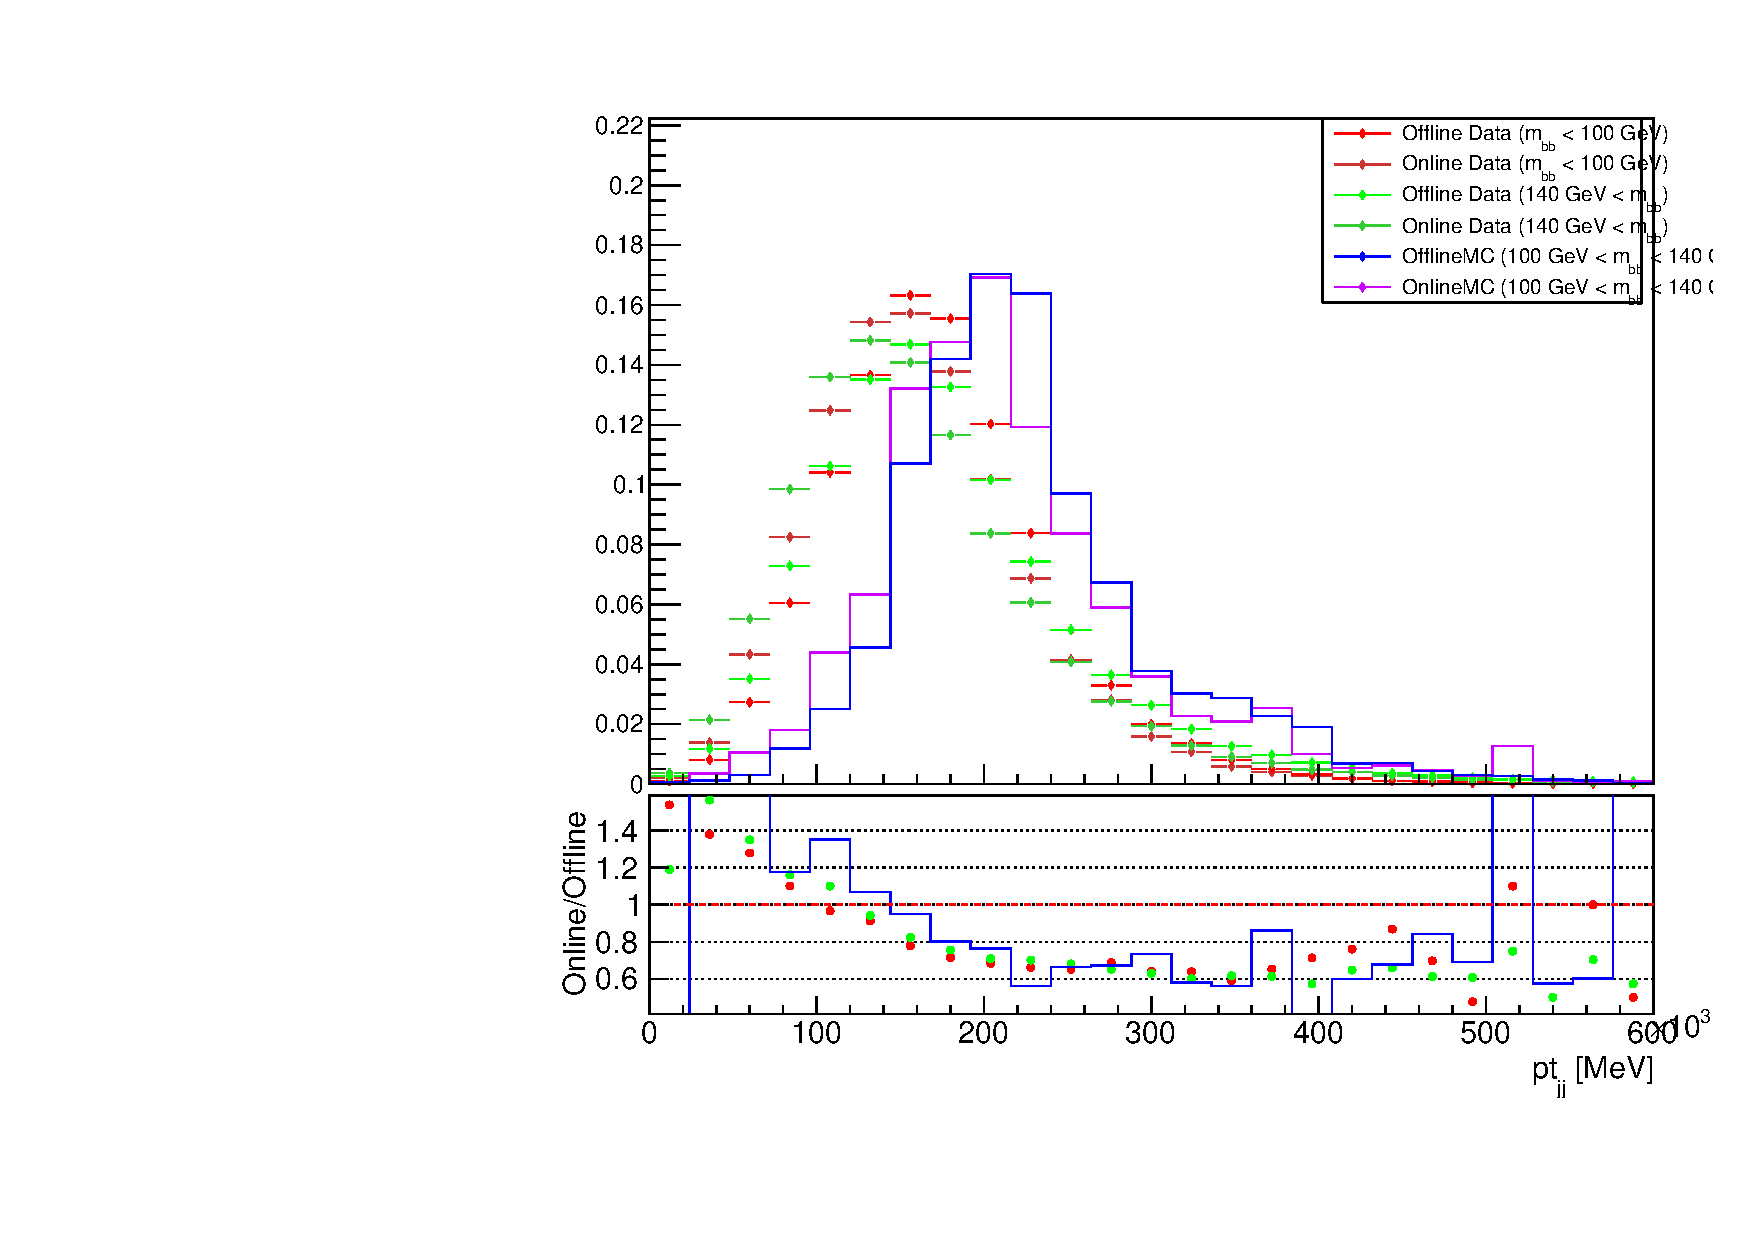
\includegraphics[width=1\linewidth]{ptjj}
				\caption{}
				\label{fig:bdtptjj}
			\end{minipage}
		\end{figure}
		
		\begin{figure}[h]
			\centering
			\begin{minipage}[h]{0.45\linewidth}
				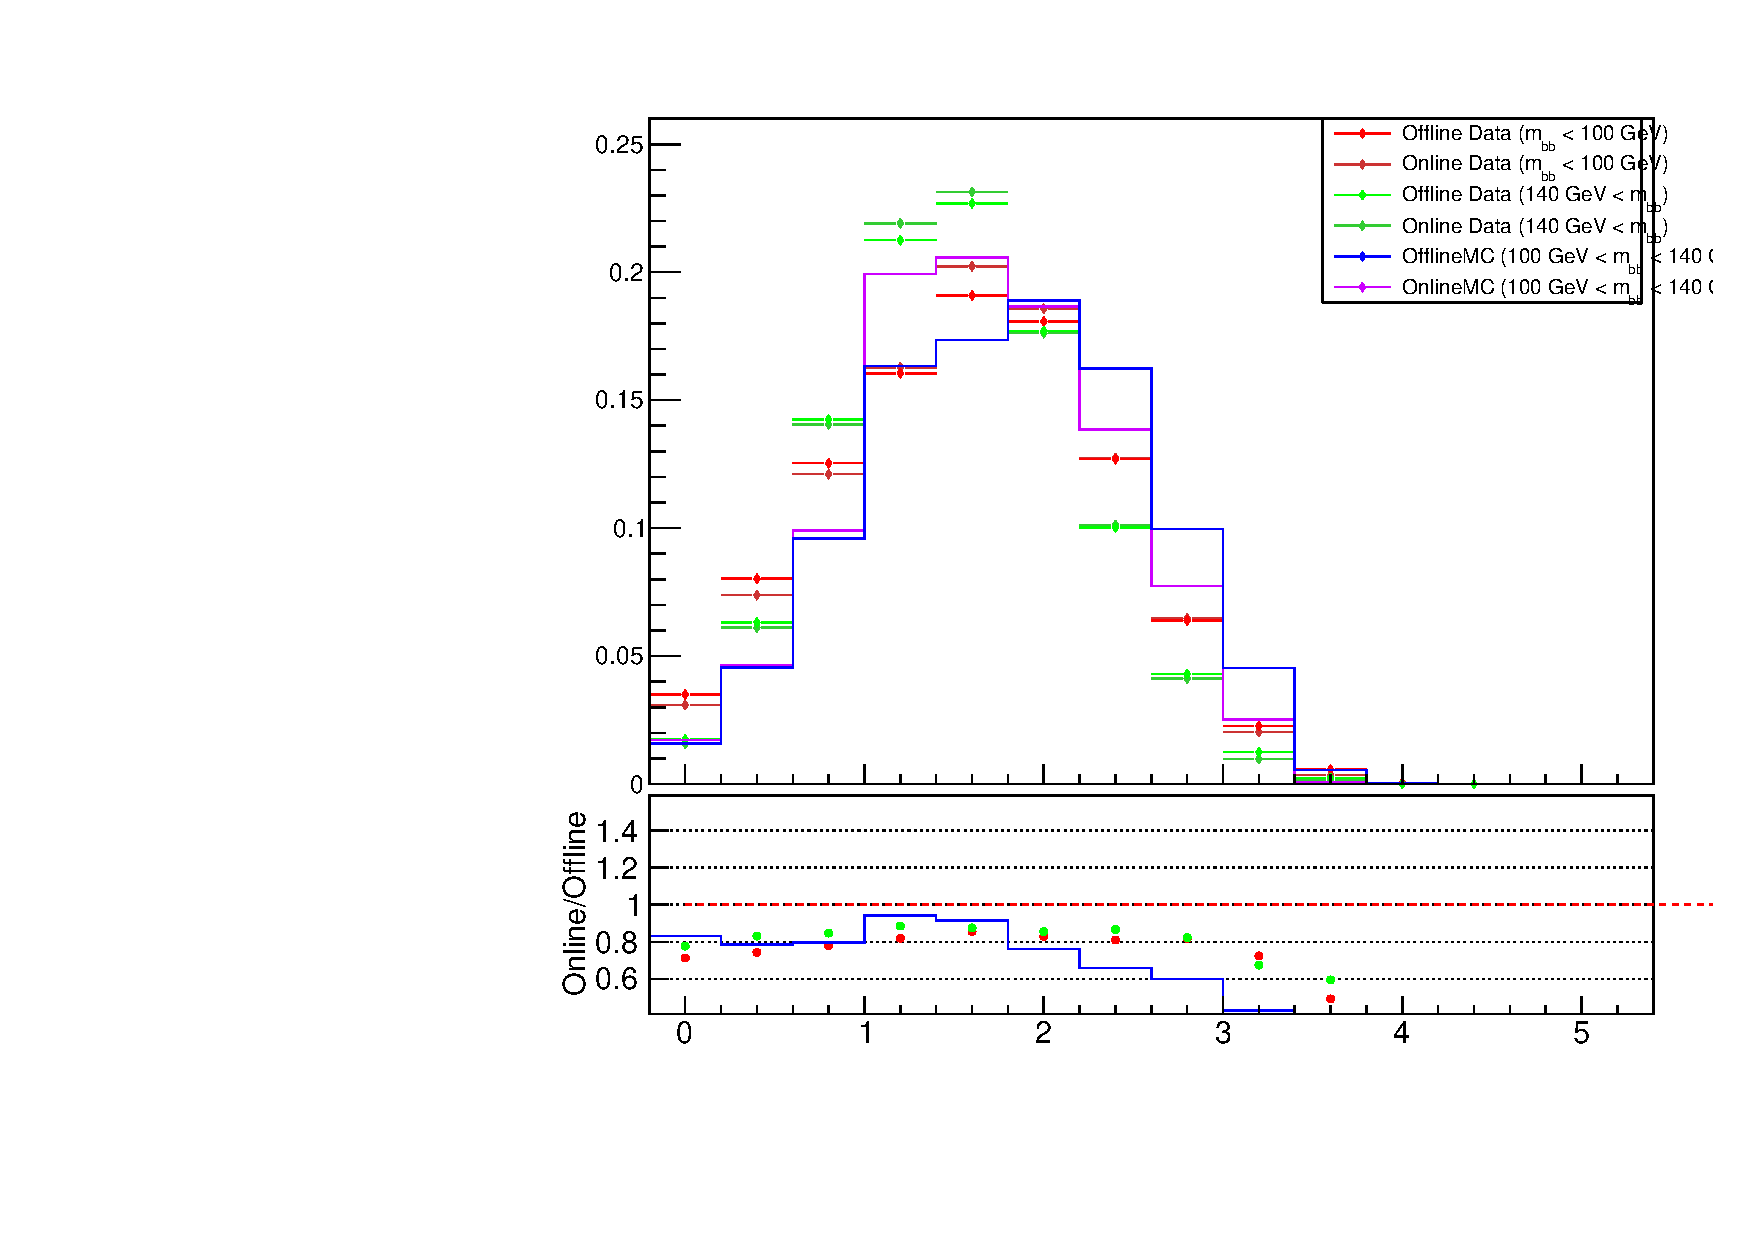
\includegraphics[width=1\linewidth]{etastar}
				\caption{}
				\label{fig:bdtetastar}
			\end{minipage}
			\quad
			\begin{minipage}[h]{0.45\linewidth}
				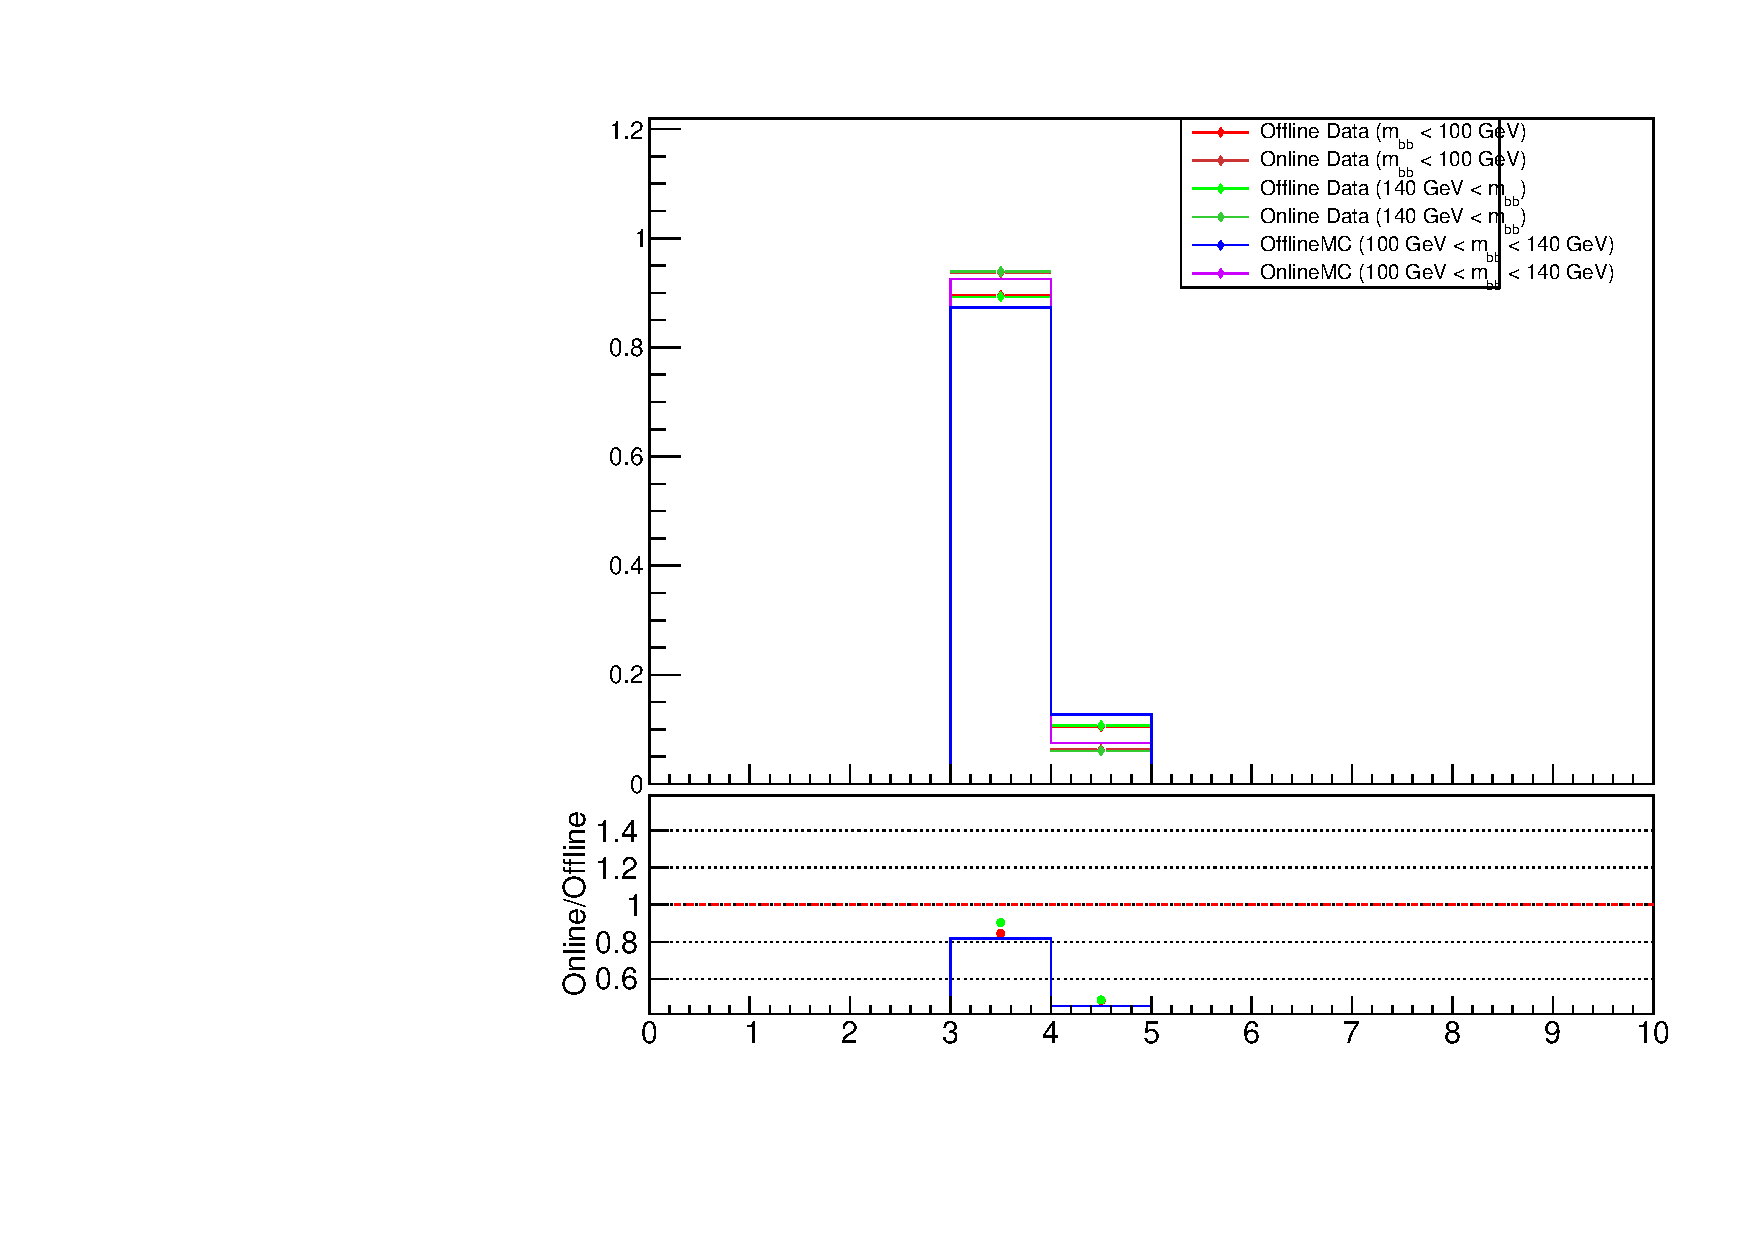
\includegraphics[width=1\linewidth]{maxeta}
				\caption{}
				\label{fig:bdtmaxeta}
			\end{minipage}
		\end{figure}
		
		\begin{figure}[h]
			\centering
			\begin{minipage}[h]{0.45\linewidth}
				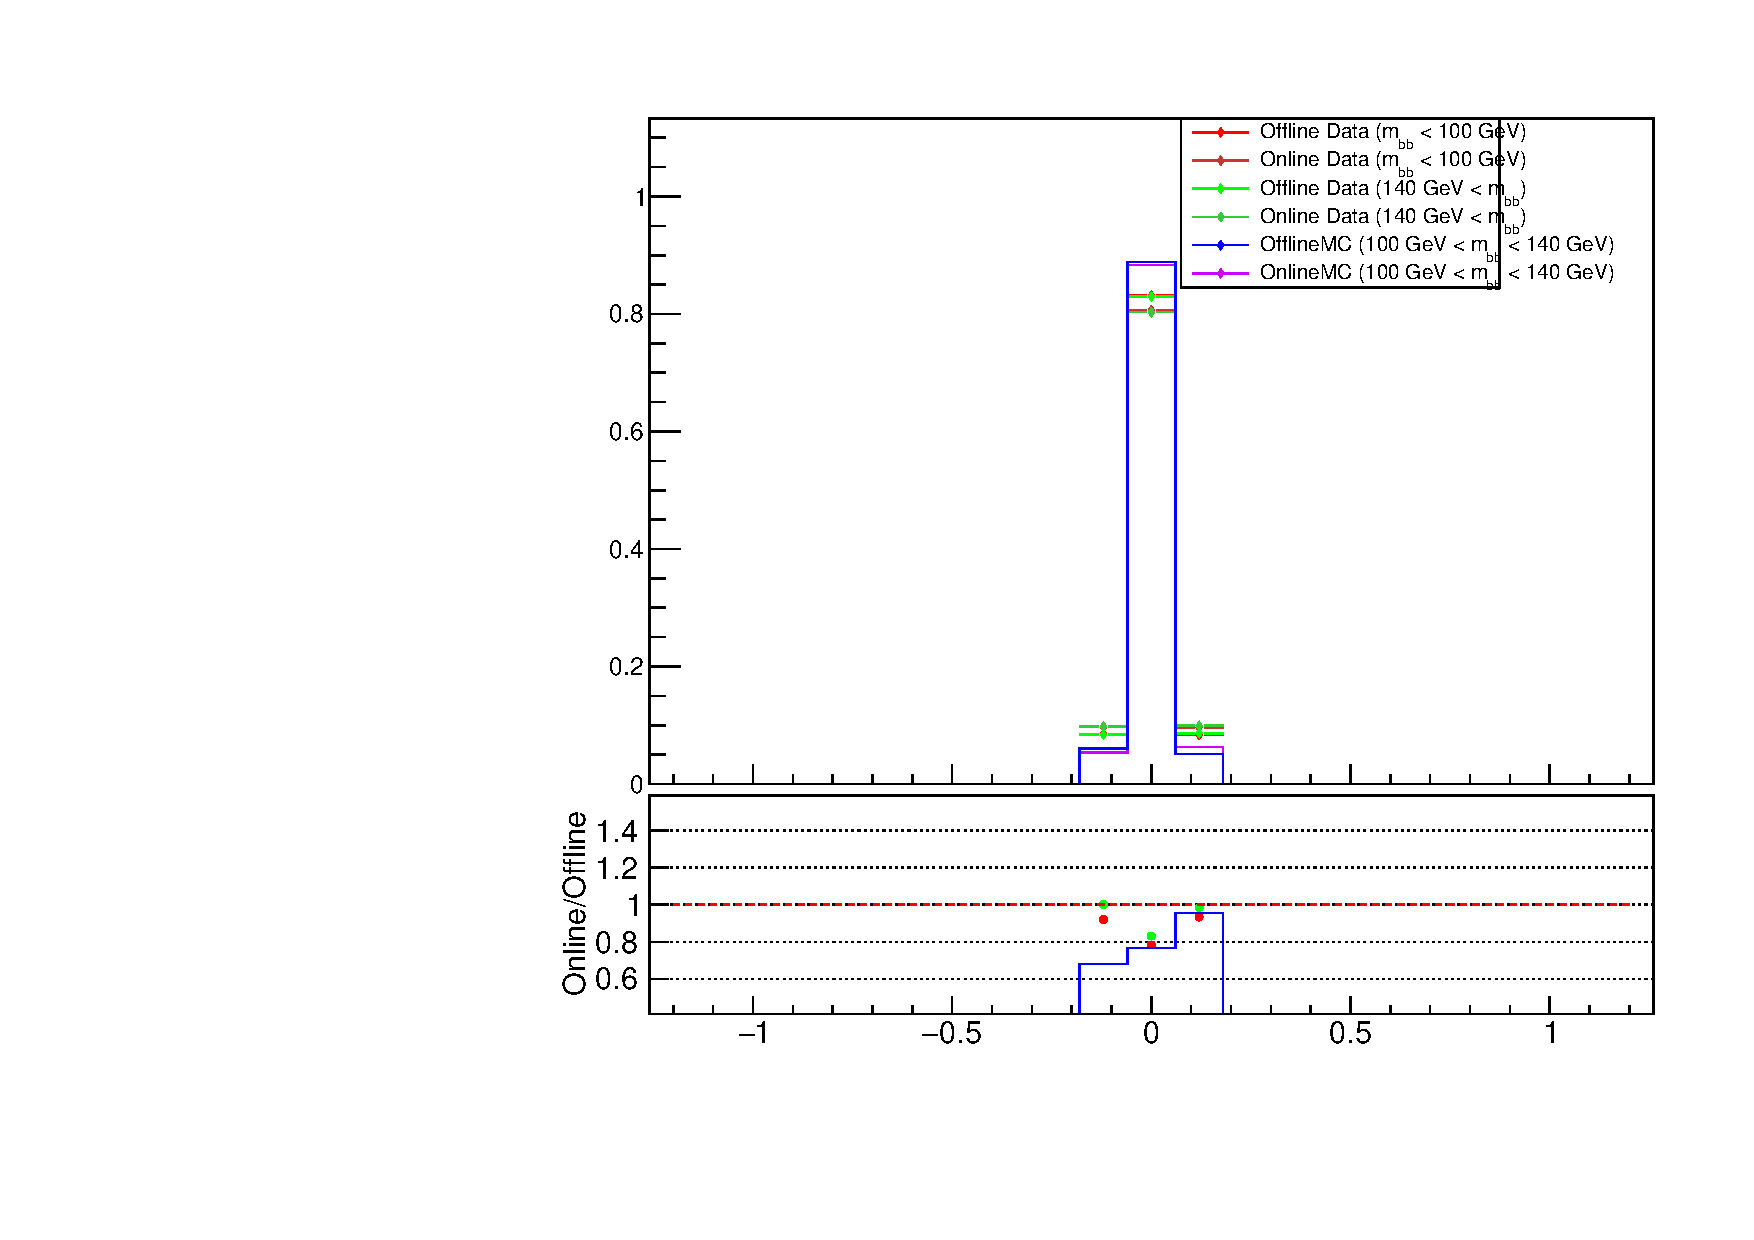
\includegraphics[width=1\linewidth]{costheta}
				\caption{}
				\label{fig:bdtcpostheta}
			\end{minipage}
			\quad
			\begin{minipage}[h]{0.45\linewidth}
				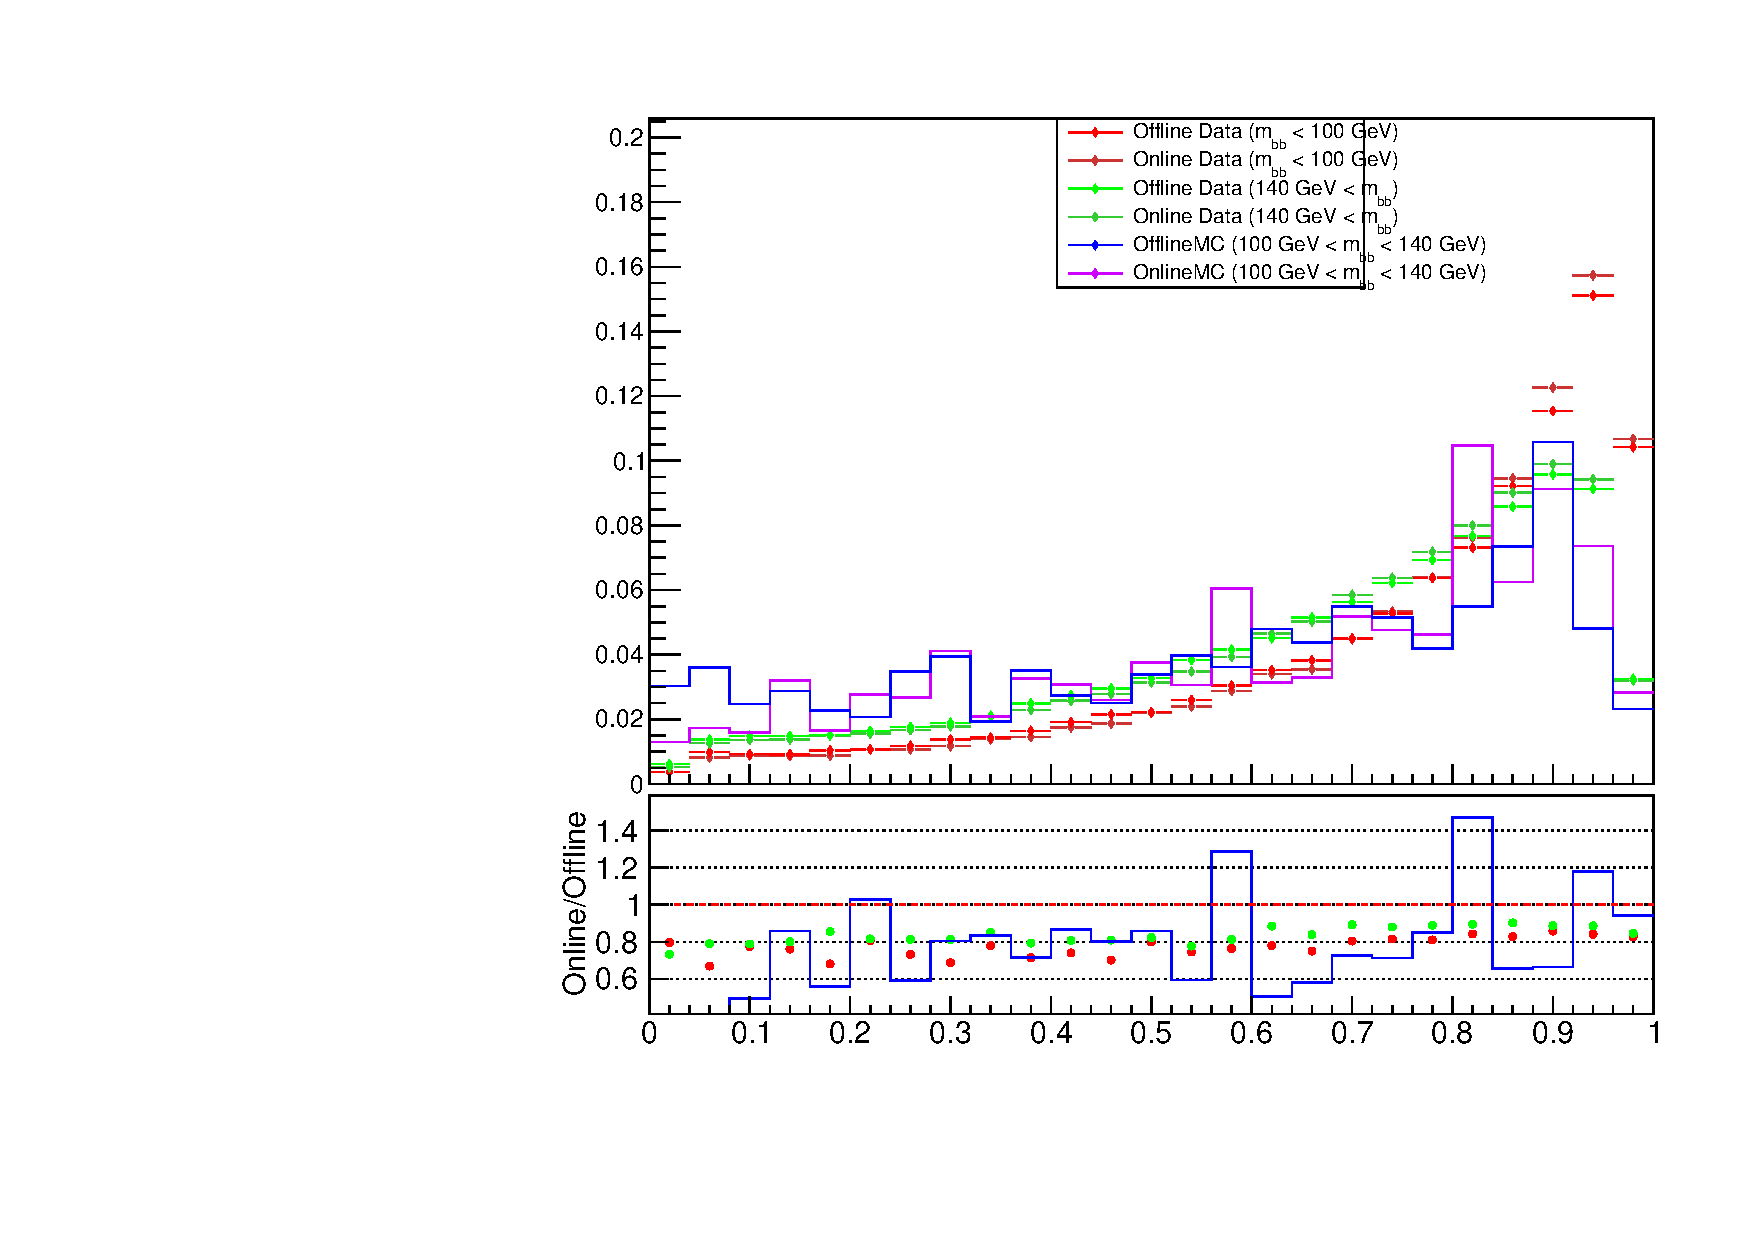
\includegraphics[width=1\linewidth]{ptbalance}
				\caption{}
				\label{fig:bdtptbalance}
			\end{minipage}
		\end{figure}


\section{Mbb Distribution}

		\begin{figure}[h]
			\centering
			\begin{minipage}[h]{0.45\linewidth}
				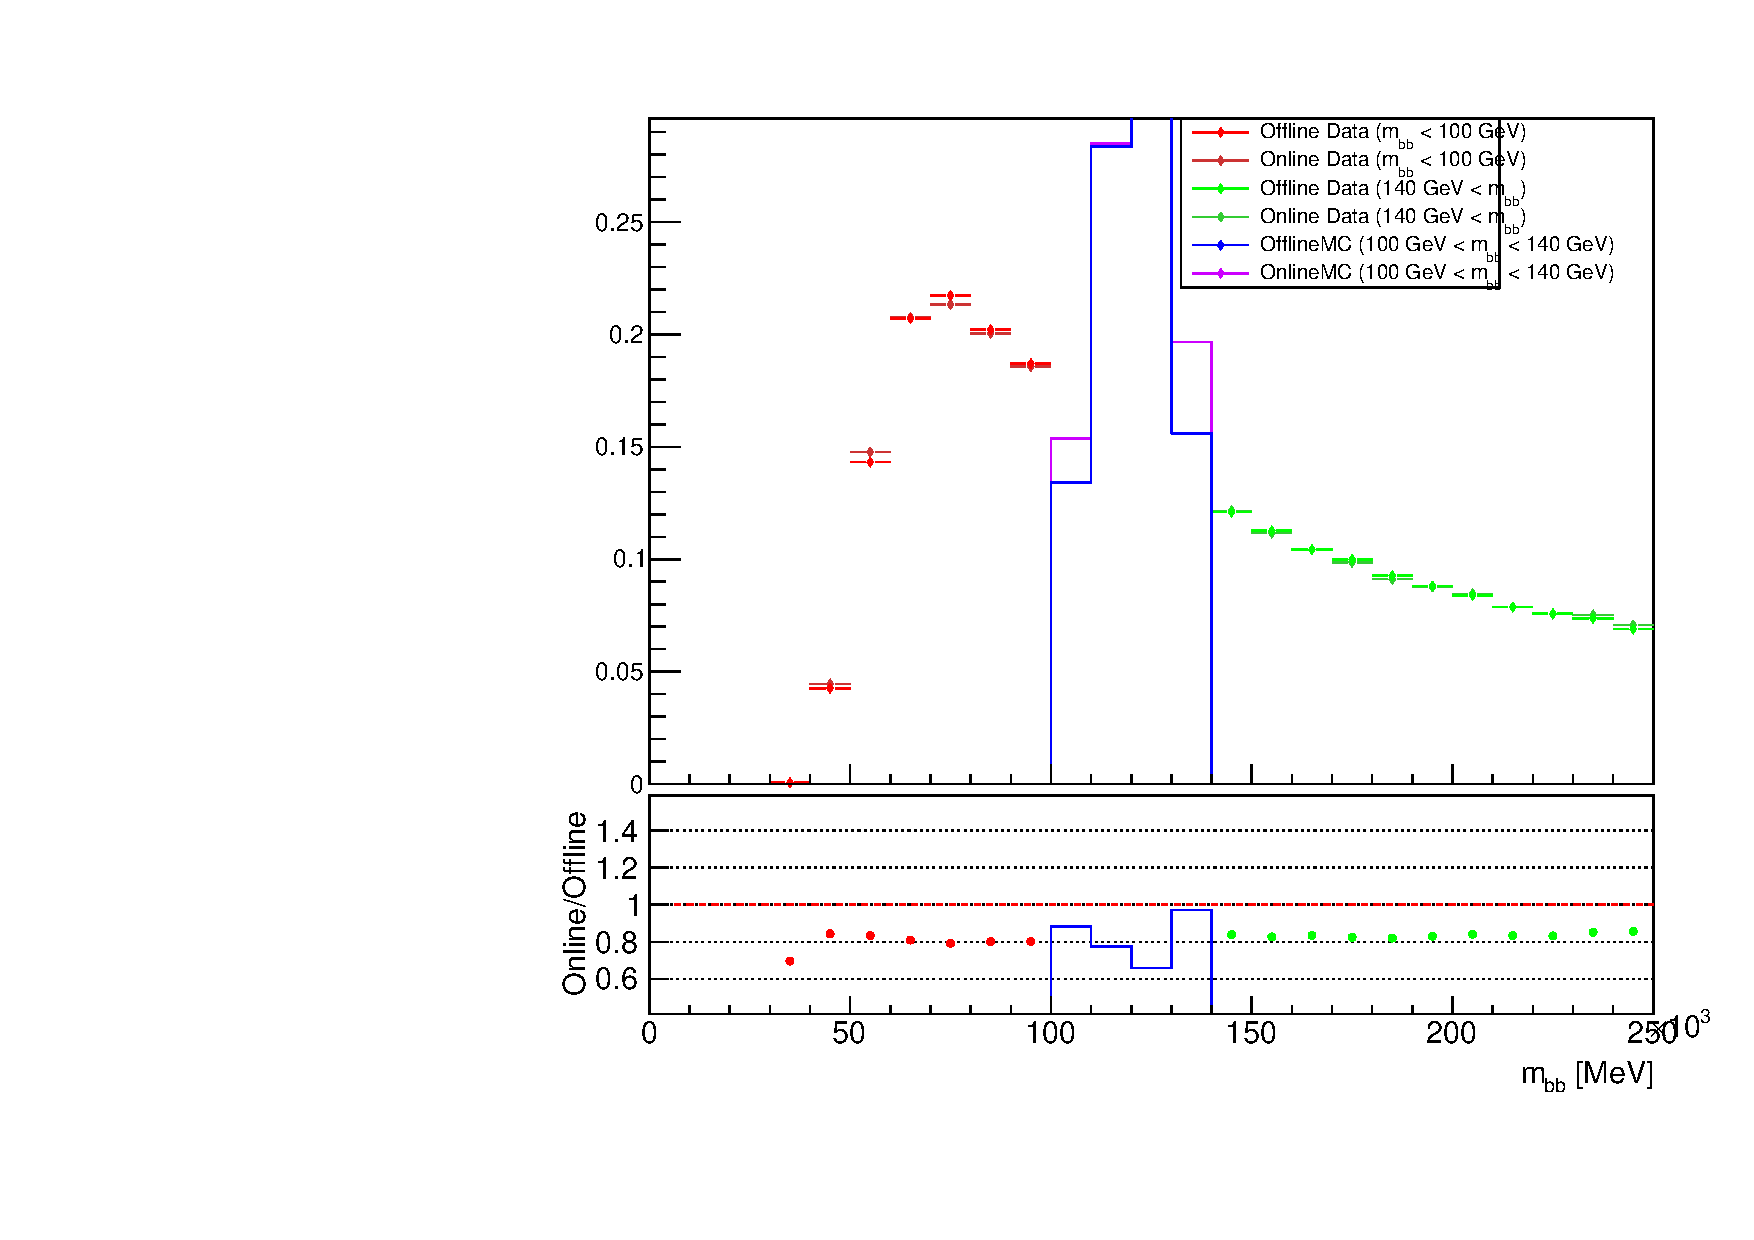
\includegraphics[width=1\linewidth]{mbb}
				\caption{}
				\label{fig:bdtmbb}
			\end{minipage}
			\quad
			\begin{minipage}[h]{0.45\linewidth}
				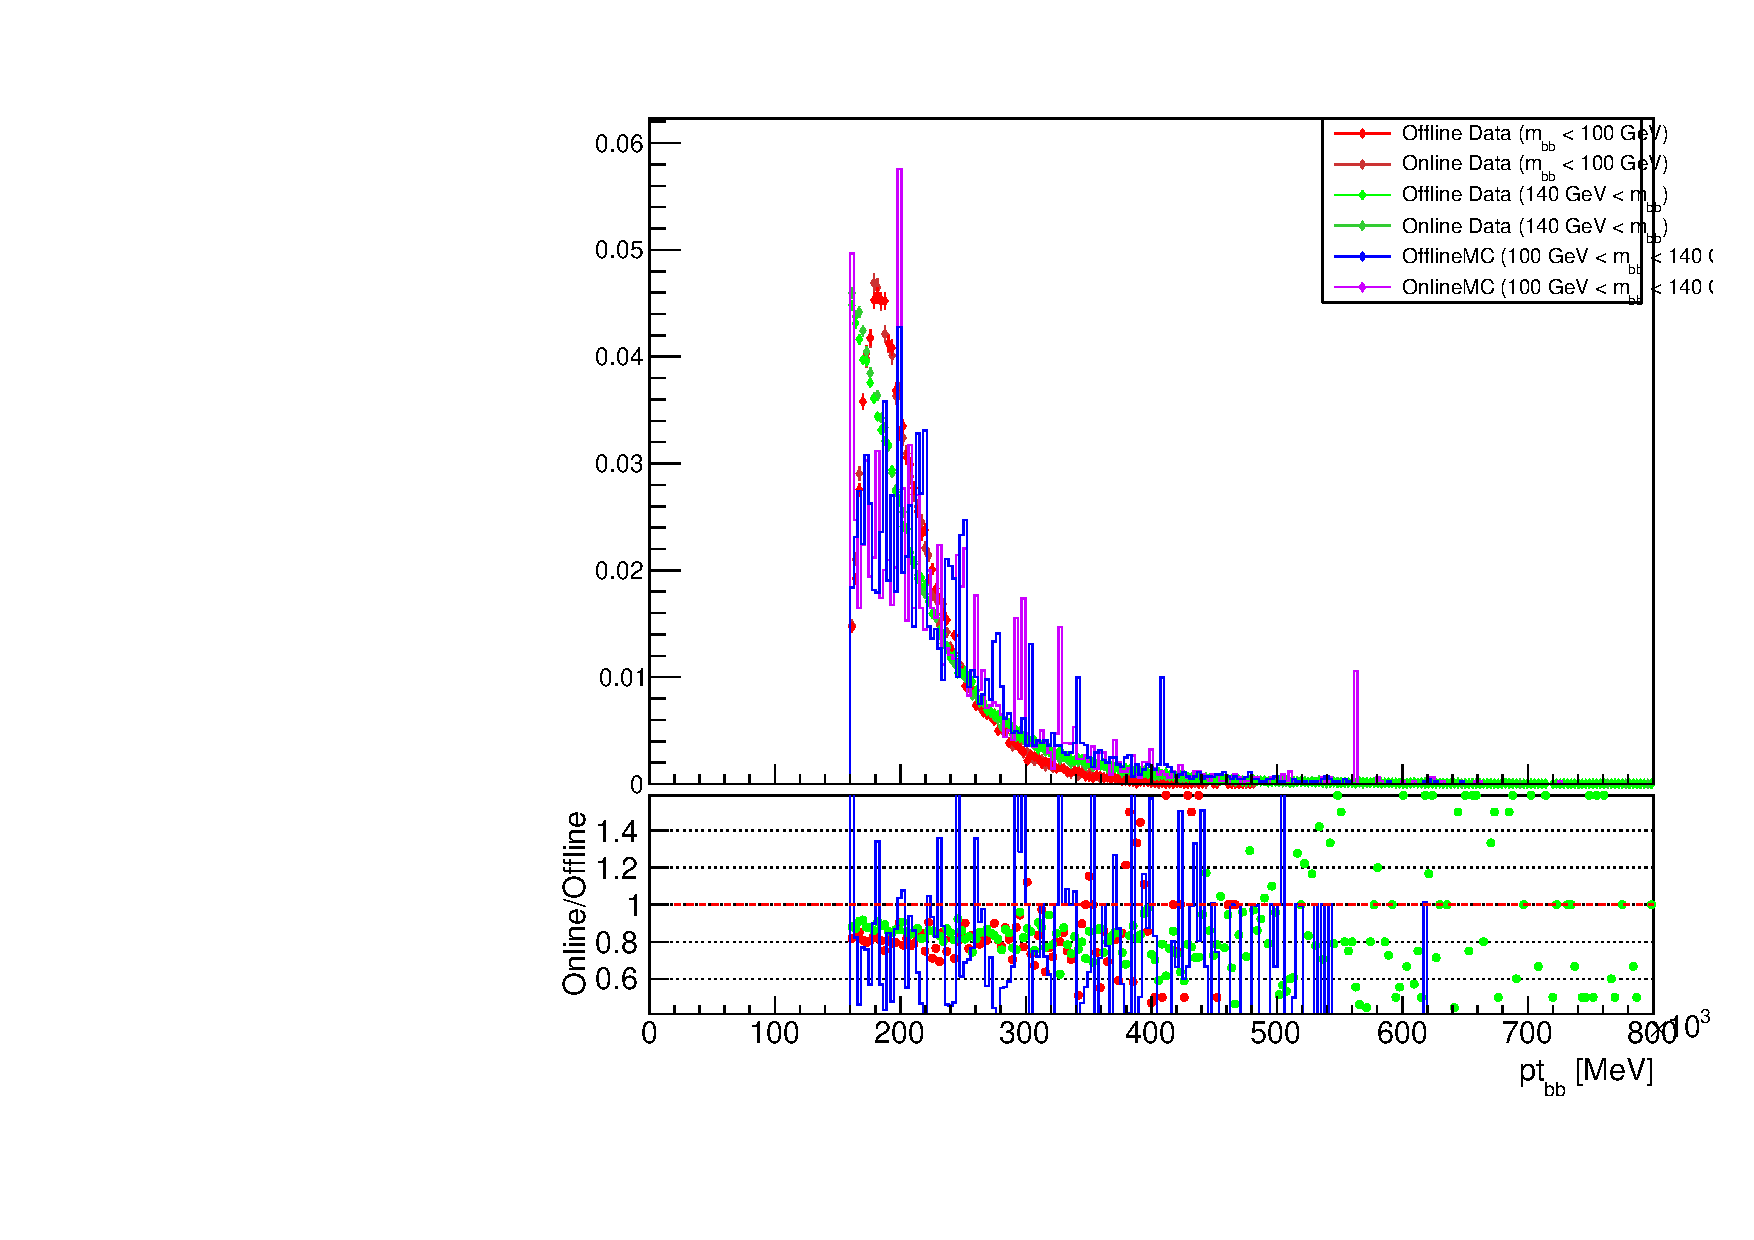
\includegraphics[width=1\linewidth]{ptbb}
				\caption{}
				\label{fig:bdtptbb}
			\end{minipage}
		\end{figure}

	Prior paper suggests this is the 'final' plot, a shape comparison between BDT influenced control and signal regions of the Mbb distribution. A little confused as to exactly what we need here.

\endinput
